% A LaTeX template for MSc Thesis submissions to
% Politecnico di Milano (PoliMi) - School of Industrial and Information Engineering
%
% S. Bonetti, A. Gruttadauria, G. Mescolini, A. Zingaro
% e-mail: template-tesi-ingind@polimi.it
%
% Last Revision: October 2021
%
% Copyright 2021 Politecnico di Milano, Italy. NC-BY

\documentclass{Configuration_Files/PoliMi3i_thesis}

%------------------------------------------------------------------------------
%	REQUIRED PACKAGES AND  CONFIGURATIONS
%------------------------------------------------------------------------------

% CONFIGURATIONS
\usepackage{parskip} % For paragraph layout
\usepackage{setspace} % For using single or double spacing
\usepackage{emptypage} % To insert empty pages
\usepackage{multicol} % To write in multiple columns (executive summary)
\setlength\columnsep{15pt} % Column separation in executive summary
\setlength\parindent{0pt} % Indentation
\raggedbottom

% PACKAGES FOR TITLES
\usepackage{titlesec}
% \titlespacing{\section}{left spacing}{before spacing}{after spacing}
\titlespacing{\section}{0pt}{3.3ex}{2ex}
\titlespacing{\subsection}{0pt}{3.3ex}{1.65ex}
\titlespacing{\subsubsection}{0pt}{3.3ex}{1ex}
\usepackage{color}

% PACKAGES FOR LANGUAGE AND FONT
\usepackage[english]{babel} % The document is in English
\usepackage[utf8]{inputenc} % UTF8 encoding
\usepackage[T1]{fontenc} % Font encoding
\usepackage[11pt]{moresize} % Big fonts

% PACKAGES FOR IMAGES
\usepackage{graphicx}
\usepackage{transparent} % Enables transparent images
\usepackage{eso-pic} % For the background picture on the title page
\usepackage{subfig} % Numbered and caption subfigures using \subfloat.
\usepackage{tikz} % A package for high-quality hand-made figures.
\usetikzlibrary{}
\graphicspath{{./Images/}} % Directory of the images
\usepackage{caption} % Coloured captions
\usepackage{xcolor} % Coloured captions
\usepackage{amsthm,thmtools,xcolor} % Coloured "Theorem"
\usepackage{float}

% STANDARD MATH PACKAGES
\usepackage{amsmath}
\usepackage{amsthm}
\usepackage{amssymb}
\usepackage{amsfonts}
\usepackage{bm}
\usepackage[overload]{empheq} % For braced-style systems of equations.
\usepackage{fix-cm} % To override original LaTeX restrictions on sizes

% PACKAGES FOR TABLES
\usepackage{tabularx}
\usepackage{longtable} % Tables that can span several pages
\usepackage{colortbl}

% PACKAGES FOR ALGORITHMS (PSEUDO-CODE)
\usepackage{algorithm}
\usepackage{algorithmic}

% PACKAGES FOR REFERENCES & BIBLIOGRAPHY
\usepackage[colorlinks=true,linkcolor=black,anchorcolor=black,citecolor=black,filecolor=black,menucolor=black,runcolor=black,urlcolor=black]{hyperref} % Adds clickable links at references
\usepackage{cleveref}
\usepackage[square, numbers, sort&compress]{natbib} % Square brackets, citing references with numbers, citations sorted by appearance in the text and compressed
\bibliographystyle{abbrvnat} % You may use a different style adapted to your field

% OTHER PACKAGES
\usepackage{pdfpages} % To include a pdf file
\usepackage{afterpage}
\usepackage{lipsum} % DUMMY PACKAGE
\usepackage{fancyhdr} % For the headers
\fancyhf{}

% Input of configuration file. Do not change config.tex file unless you really know what you are doing.
% Define blue color typical of polimi
\definecolor{bluepoli}{cmyk}{0.4,0.1,0,0.4}

% Custom theorem environments
\declaretheoremstyle[
  headfont=\color{bluepoli}\normalfont\bfseries,
  bodyfont=\color{black}\normalfont\itshape,
]{colored}

% Set-up caption colors
\captionsetup[figure]{labelfont={color=bluepoli}} % Set colour of the captions
\captionsetup[table]{labelfont={color=bluepoli}} % Set colour of the captions
\captionsetup[algorithm]{labelfont={color=bluepoli}} % Set colour of the captions

\theoremstyle{colored}
\newtheorem{theorem}{Theorem}[chapter]
\newtheorem{proposition}{Proposition}[chapter]

% Enhances the features of the standard "table" and "tabular" environments.
\newcommand\T{\rule{0pt}{2.6ex}}
\newcommand\B{\rule[-1.2ex]{0pt}{0pt}}

% Pseudo-code algorithm descriptions.
\newcounter{algsubstate}
\renewcommand{\thealgsubstate}{\alph{algsubstate}}
\newenvironment{algsubstates}
  {\setcounter{algsubstate}{0}%
   \renewcommand{\STATE}{%
     \stepcounter{algsubstate}%
     \Statex {\small\thealgsubstate:}\space}}
  {}

% New font size
\newcommand\numfontsize{\@setfontsize\Huge{200}{60}}

% Title format: chapter
\titleformat{\chapter}[hang]{
\fontsize{50}{20}\selectfont\bfseries\filright}{\textcolor{bluepoli} \thechapter\hsp\hspace{2mm}\textcolor{bluepoli}{|   }\hsp}{0pt}{\huge\bfseries \textcolor{bluepoli}
}

% Title format: section
\titleformat{\section}
{\color{bluepoli}\normalfont\Large\bfseries}
{\color{bluepoli}\thesection.}{1em}{}

% Title format: subsection
\titleformat{\subsection}
{\color{bluepoli}\normalfont\large\bfseries}
{\color{bluepoli}\thesubsection.}{1em}{}

% Title format: subsubsection
\titleformat{\subsubsection}
{\color{bluepoli}\normalfont\large\bfseries}
{\color{bluepoli}\thesubsubsection.}{1em}{}

% Shortening for setting no horizontal-spacing
\newcommand{\hsp}{\hspace{0pt}}

\makeatletter
% Renewcommand: cleardoublepage including the background pic
\renewcommand*\cleardoublepage{%
  \clearpage\if@twoside\ifodd\c@page\else
  \null
  \AddToShipoutPicture*{\BackgroundPic}
  \thispagestyle{empty}%
  \newpage
  \if@twocolumn\hbox{}\newpage\fi\fi\fi}
\makeatother

%For correctly numbering algorithms
\numberwithin{algorithm}{chapter}

%----------------------------------------------------------------------------
%	NEW COMMANDS DEFINED
%----------------------------------------------------------------------------

% EXAMPLES OF NEW COMMANDS
\newcommand{\bea}{\begin{eqnarray}} % Shortcut for equation arrays
\newcommand{\eea}{\end{eqnarray}}
\newcommand{\e}[1]{\times 10^{#1}}  % Powers of 10 notation

%----------------------------------------------------------------------------
%	ADD YOUR PACKAGES (be careful of package interaction)
%----------------------------------------------------------------------------

%----------------------------------------------------------------------------
%	ADD YOUR DEFINITIONS AND COMMANDS (be careful of existing commands)
%----------------------------------------------------------------------------

%----------------------------------------------------------------------------
%	BEGIN OF YOUR DOCUMENT
%----------------------------------------------------------------------------

\begin{document}

\fancypagestyle{plain}{%
\fancyhf{} % Clear all header and footer fields
\fancyhead[RO,RE]{\thepage} %RO=right odd, RE=right even
\renewcommand{\headrulewidth}{0pt}
\renewcommand{\footrulewidth}{0pt}}

%----------------------------------------------------------------------------
%	TITLE PAGE
%----------------------------------------------------------------------------

\pagestyle{empty} % No page numbers
\frontmatter % Use roman page numbering style (i, ii, iii, iv...) for the preamble pages

\puttitle{
        title=Software Engineering 2\\Requirements Analysis and\\Specification Document,
        name1=Filippo Balzarini - , % Author Name and Surname
        name2=Christian Biffi - ,
        name3=Michele Cavicchioli - ,
        academicyear=2023-2024,
        date=31-January-2016,
        copyright=Copyright © 2023 Filippo Balzarini Christian Biffi Michele Cavicchioli – All rights reserved,
        download page=https://github.com/filomba01/BalzariniBiffiCavicchioli,
    }

%\puttitle{
%    Deliverable=RASD,
%	title=Requirement Analysis and Verification Document, % Title of the thesis
%	Authors=Filippo Balzarini Christian Biffi Michele Cavicchioli, % Author Name and Surname
%	Version=1.0,
	%advisor= Prof. Name Surname, % Supervisor name
	%coadvisor={Name Surname, Name Surname}, % Co-Supervisor name, remove this line if there is none
    %cycle={cicle phd},
    %tutor=Prof. Name Surname,
    %phdcycle = {Year 2023 - XXXV Cycle}
 %   Date=31-January-2016,
 %   Copyright=Copyright © 2023 Filippo Balzarini Christian Biffi Michele Cavicchioli – All rights reserved,
 %   Download page=https://github.com/filomba01/BalzariniBiffiCavicchioli,
    %chair={piroddi}
%} % These info will be put into your Title page


%----------------------------------------------------------------------------
%	PREAMBLE PAGES: ABSTRACT (inglese e italiano), EXECUTIVE SUMMARY
%----------------------------------------------------------------------------
\startpreamble
\setcounter{page}{1} % Set page counter to 1




%----------------------------------------------------------------------------
%	LIST OF CONTENTS/FIGURES/TABLES/SYMBOLS
%----------------------------------------------------------------------------

% TABLE OF CONTENTS
\thispagestyle{empty}
\tableofcontents % Table of contents
\thispagestyle{empty}
\cleardoublepage

%-------------------------------------------------------------------------
%	THESIS MAIN TEXT
%-------------------------------------------------------------------------
% In the main text of your thesis you can write the chapters in two different ways:
%
%(1) As presented in this template you can write:
%    \chapter{Title of the chapter}
%    *body of the chapter*
%
%(2) You can write your chapter in a separated .tex file and then include it in the main file with the following command:
%    \chapter{Title of the chapter}
%    \input{chapter_file.tex}
%
% Especially for long thesis, we recommend you the second option.

\addtocontents{toc}{\vspace{2em}} % Add a gap in the Contents, for aesthetics
\mainmatter % Begin numeric (1,2,3...) page numbering

%-------------------------------------------------------------------------
%	Introduction
%-------------------------------------------------------------------------
\chapter{Introduction}
\label{ch:introduction}%
\renewcommand{\arraystretch}{1.5} % Adjust the multiplier as needed

\section{Purpose}
\label{s:Purpose}%

The CodeKata is a learning method that takes inspiration from the Kata techniques and is based on continuous practice which became very popular in those years.

CodeKataBattle delineates an innovative platform geared towards enhancing students' software development skills through collaborative learning using CodeKata’s fundamentals. Facilitated by educators, CKB provides a dynamic environment where students engage in code kata battles, refining their programming proficiency and embracing best practices such as the test-driven development approach.

Similar to recent initiatives addressing global challenges, CKB empowers educators to orchestrate challenges within competition, stimulating healthy competition and cultivating an environment for skill enhancement. The platform enables educators to define battle parameters, set deadlines, and configure scoring criteria, fostering a tailored and effective learning experience.

At its core, a code kata battle presents students with programming challenges within specific language frameworks, coupled with exhaustive test cases. Teams collaboratively tackle these exercises, adhering to a test-first methodology and submitting solutions to the platform upon battle completion.

CKB's automated evaluation system ensures an impartial assessment of student submissions. Automated scrutiny covers mandatory factors, including functional aspects, timeliness, and source code quality, offering an unbiased representation of team performance. Educators can further enhance evaluations with optional manual assessments, providing nuanced insights into student work.

\pagebreak

\subsection{Goals}
\label{ss:goals}%
The platform will be used by two types of users: Educators (ED) and Students (ST). The ED will be able to create competitions and battles within competitions. The ST will be able to create teams and join battles as a team or individually. The platform will communicate with Github to pull the latest code submission and provides automated evaluation of the code submitted. The platform will also show a ranking of the competition and battles.

Below there is the table of goals that the platform will achieve:
\begin{longtable}{|l|l|}
  \hline
  \textbf{\#} & \textbf{Goal}      \\
  \hline
  G1 & Enable ED to manage competitions \\
  \hline
  G2 & Enable ED to manage code battles within competitions \\
  \hline
  G3 & Enable ST to participate in a competition \\
  \hline
  G4 & Enable ST to be part of a team within a battle \\
  \hline
  G5 & Send Notifications to STs   \\
  \hline
  G6 & Automatically create GitHub repositories for every battle in a competition    \\
  \hline
  G7 & Synchronize the submission of each candidate with their GitHub repository   \\
  \hline
  G8 & CKB provides an evaluation of the code submitted    \\
  \hline
  G9 & Allow users to view rankings in both battles and competitions   \\
  \hline
  G10 & Allow to assign badges to the students    \\
  \hline
  \caption{List of goals}
  \label{tab:goals}
\end{longtable}

\pagebreak
\section{Scope}
\label{s:Scope}%

\subsection{World phenomena}
\label{ss:world_phenomena}%

\begin{table}[H]
  \begin{tabular}{|l|l|}

    \hline
    \textbf{ID} & \textbf{Definitions}      \\
    \hline
    WP1 & ED wants to create a competitions \\
    \hline
    WP2 & ED wants to create a battle \\
    \hline
    WP3 & ST wants to participate in a competition \\
    \hline
    WP4 & ST wants to participate in a battle     \\
    \hline
    WP5 & ST set up GitHub actions    \\
    \hline
    
  \end{tabular}
  \caption{List of the world phenomena}
  \label{tab:worldPhenomena}
\end{table}

\subsection{Shared phenomena}
\label{ss:shared_phenomena}%

\begin{longtable}{|l|l|}

  \hline
  \textbf{ID} & \textbf{Definitions}      \\
  \hline
  SP1 & ST creates an account on the platform \\
  \hline
  SP2 & ED creates an account in the platform \\
  \hline
  SP3 & ST logs in to the platform \\
  \hline
  SP4 & ED logs in to the platform  \\
  \hline
  SP5 & ST registers for the competitions before the deadline   \\
  \hline
  SP6 & ED creates a badge with certain rules   \\
  \hline
  SP7 & ED manually evaluates the code submitted by students   \\
  \hline
  SP8 & ED creates a competition   \\
  \hline
  SP9 & ED creates a battle within a competition   \\
  \hline
  SP10 & ED closes a competition   \\
  \hline
  SP11 & ST pushes new commit(s) into their GitHub repository before the deadline   \\
  \hline
  SP12 & ST invites other STs to participate in a battle as a team   \\
  \hline
  SP13 & ST subscribes as a single/team for an incoming battle before the deadline   \\
  \hline
  SP14 & CKB sends a notification that a competition is available to ST   \\
  \hline
  SP15 & CKB sends a notification that a battle is created inside a competition to ST   \\
  \hline
  SP16 & CKB sends a notification that a competition has ended to ST   \\
  \hline
  SP17 & CKB sends a notification that a battle has ended to ST   \\
  \hline
  SP18 & CKB sends links to the GitHub repository to all the ST subscribed   \\
  \hline
  SP19 & CKB updates scores for each ST   \\
  \hline
  SP20 & CKB gives badge to ST   \\
  \hline
  SP21 & CKB updates the ranking of the competition   \\
  \hline
  SP22 & CKB updates the ranking of the battle   \\
  \hline
  
  \caption{List of the shared phenomena}
  \label{tab:sharedPhenomena}
\end{longtable}


\section{Definitions, Acronyms, Abbreviations}
\label{s:Definitions_Acronyms_Abbreviations}%

\subsection{Definitions}
\label{ss:Definitions}

\begin{table}[H]
  \begin{tabular}{|l|l|}

    \hline
    User & Anyone interacting with the system, it can be both a Student or an Educator    \\
    \hline
    Manage & Create, supervise and edit a certain element of the application. \\
    \hline
  \end{tabular}
  \caption{List of definitions}
  \label{tab:definitions}
\end{table}

\subsection{Acronyms}
\label{ss:Acronyms}

\begin{table}[H]
  \begin{tabular}{|l|l|}

    \hline
    ST & Student \\
    \hline
    ED & Educator \\
    \hline
    CKB & CodaKataBattle \\
    \hline
    RASD & Requirements Analysis and Specification Document     \\
    \hline
    SAT & Static Analyzer Tool    \\
    \hline
    T & Team    \\
    \hline
  \end{tabular}
  \caption{List of Acronyms}
  \label{tab:acronyms}
\end{table}

\subsection{Abbreviations}
\label{ss:Abbreviations}


\begin{table}[H]
  \begin{tabular}{|l|l|}

    \hline
    WPX & World Phenomena X    \\
    \hline
    SPX & Shared Phenomena X    \\
    \hline
    GX & Goal Number X    \\
    \hline
    DX & Domain Assumption X    \\
    \hline
    UCX & Use Case X    \\
    \hline

  \end{tabular}
  \caption{List of abbreviations}
  \label{tab:abbreviations}
\end{table}



\section{Revision history}
\label{s:Revision_history}%


\section{Reference Documents}
\label{s:Reference_documents}%

\begin{itemize}
  \item The specification document of the project: \textit{Assignment RDD AY 2023-2024}
\end{itemize}

\section{Document Structure}
\label{s:Document_Structure}%

The document is divided in five main section described as below.

The first section is the introduction, that introduce the goals of the project, purpose and the analysis of world and shared phenomena. It also contains the definitions, acronyms and abbreviations used in the document. 

The second section is the overall description, that contains the general factors that affect the product. Here there is also the analysis of the scenarios and functions of the platform and the domain assumptions.

Then as third section there is the specific requirements section, that contains the functional and non-functional requirements of the platform. Morover, there is a more detailed analysis of the use cases and the mapping between goals and requirements. Then there is a description of the interfaces necessary for the platform to implement all the functionalities.

The fourth section is the formal analysis using Alloy. Here there is the description of the model and the world generated by the Alloy Analyzer. This section is very important to prove the correctness of the model described in the previous sections.

The last section is the effort spent by each member of the group to write this document.


%-------------------------------------------------------------------------
%	Overall Description
%-------------------------------------------------------------------------
\chapter{Overall Description}
\label{ch:Overall_description}%
% The \label{...}% enables to remove the small indentation that is generated, always leave the % symbol.
\section{Product perspective}
\label{s:Product_perspective}%

\subsection{Class Diagram}
\label{ss:class_diagram}%
Here we provide the class diagram of our system and a brief description on some of the key aspects. The very first thing to explain is the logical split of the \textit{Static Analyzer} from the rest of the system, the reason for this is that we wanted to have a system that could be more \textit{flexible} than usual. The two logical parts can be implemented in the same tier or can also be split physically in terms of devices. What does not change is that when the STs set up github actions on their repository, the server that will be called when a commit is pushed is the \textbf{\textit{SA\_Server}}, which will do the necessary checks and then sends the results to the main server (\textbf{\textit{Results API}} has this purpose), where the score will be computed. Note that the Static Analyzer can be configured from the main server by using the provided APIs in \textbf{\textit{SA\_Configuration API}} (e.g., upload the test cases…). 
As asked by the assignment we distinguished two types of users, \textbf{\textit{Students}} and \textbf{\textit{Educators}}, in order to differentiate the features the platform offers to the two. To handle the participants of a battle we decided to represent every one of them as teams, therefore we can have a team that is composed by a single student, this will be very useful when analysing such teams to understand if they meet the criteria to join a battle. The \textbf{\textit{NotificationHandler}} has the purpose of handling the notifications of the users and it provides the procedures to do just so.


% TO CHECK: link educator -> competition label "creates" should it be "manages"
\begin{center}
  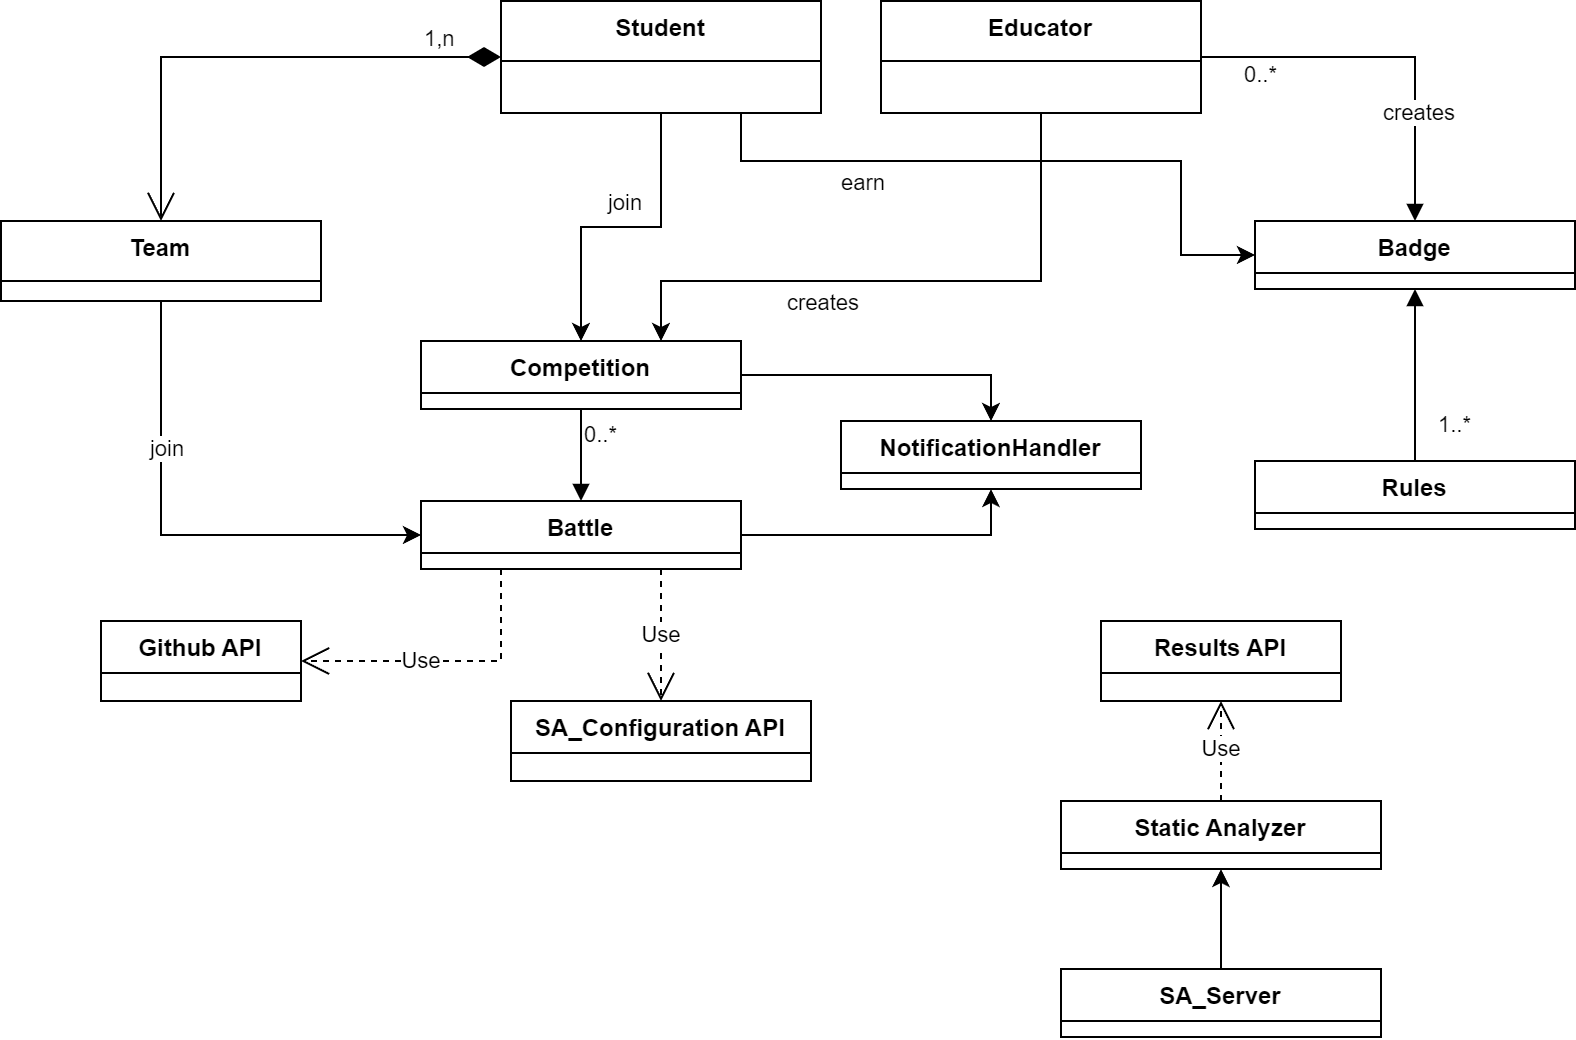
\includegraphics[width=\textwidth]{RASD_UML.png}
\end{center}

\subsection{State Diagrams}
\label{ss:state_diagrams}%

\subsubsection*{Commit in github repository}
Here there is the state diagram related to the system that processes the push of a commit in a ST repository.
  \begin{center}
    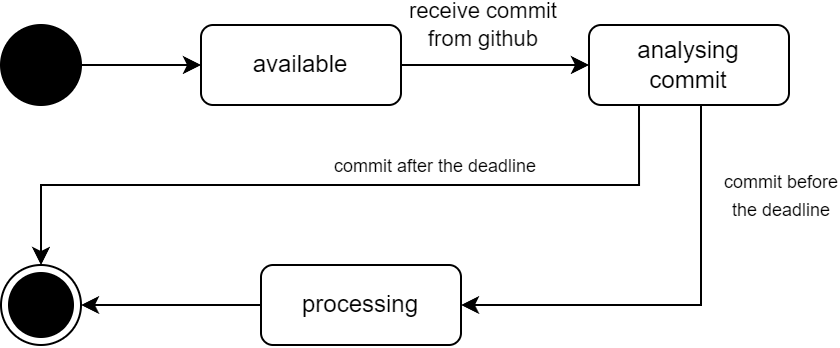
\includegraphics[width=0.6\textwidth]{StateDiagrams/SD_1.png}
  \end{center}
\newpage 
\subsubsection*{Join battle}
Here you can find the state diagram representing the process of joining a battle from the system perspective.
  \begin{center}
    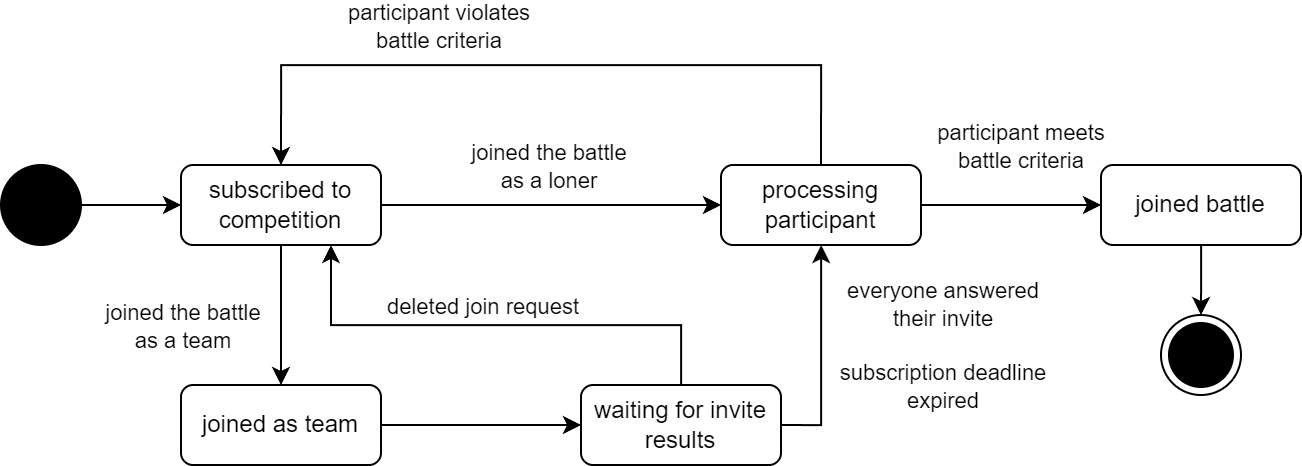
\includegraphics[width=0.8\textwidth]{StateDiagrams/SD_2.png}
  \end{center}

\subsubsection*{Accept invite to join battle}
Below you can find the state diagram representing the process of a ST accepting an invite to join a battle.
  \begin{center}
    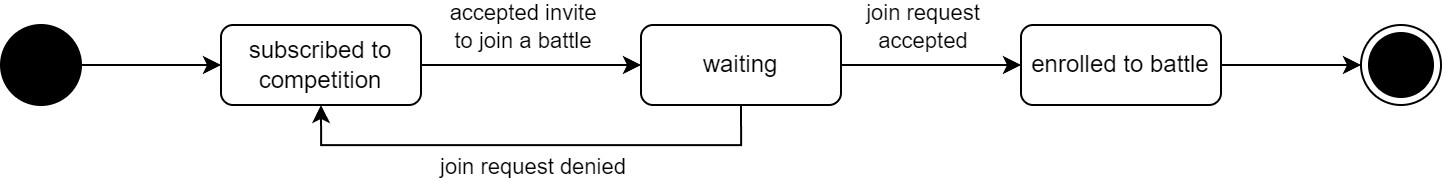
\includegraphics[width=\textwidth]{StateDiagrams/SD_3.png}
  \end{center}

  
\subsection{Scenarios}
\label{ss:scenarios}%
\subsubsection*{Scenario 1}
Professor Harry is a professor teaching at Politecnico di Milano together with professor Donald. Harry would like to encourage his students to study during the course, instead of having to study everything a few days before the exam. To do so he came up with the idea to create a challenge where the students can test their preparation and earn some extra points in the exam. While talking with other colleagues, Prof. Harry discovered CKB and he thought it was the perfect fit to implement his idea. The first thing he does is to go to the webpage of CKB and create an account by clicking the \textbf{\textit{Sign up}} button and providing some information about himself. Afterwards he is redirected to the home page of the platform where he can click the button \textbf{\textit{Create Competition}}, and finally he inserts the name of the competition and the subscription deadline. At this point he wants to invite his colleague Donald to manage the competition with him; since he is an ED in the competition he can click on \textbf{\textit{Invite Educator}} in the competition page, then provides the email of Donald's account, who will be part of the competition once he accepts the invite.

\subsubsection*{Scenario 2}
Professor Harry is an ED of a competition, within which he wants to create a battle. To do so he enters the dashboard of the competition, clicks on the button \textbf{\textit{Create Battle}} and provides everything the platform needs: description, test cases, build automation scripts, deadlines, accepted sizes of groups. Marco, a ST who subscribed to the competition, received the notitication about the newly created battle via email. Outside of the platform Marco agreed with a couple of friends to participate in the battle together. Marco then goes on the competition page and finds the newly created battle, here he finds two buttons, \textbf{\textit{Participate as: 1. Loner 2. Team}}; he clicks the second button to participate as a team and invites his friends by providing the platform his friends' account email. Once Marco's friends accepted the invite the subscription to the battle will be automatically finalized by the platform.

\subsubsection*{Scenario 3}
Professor Harry wants to give credit to the hardest working student, so while creating the competition he decided to create a new badge. The hardest working ST is the one that has written the highest amount of code lines among all the battles in the same competition. To implement this badge Prof. Harry must create a new variable \textbf{\textit{hardest\_worker}} and provide the code that defines how to compute the value of such variable. Some time after the specification of this new badge, a ST, participating in the competition and in the current battle, called Marco, pushes a commit to his repository. Since all students are supposed to setup \textit{GitHub Actions}, CKB is notified about Marco's commit, so it proceeds to run the required processes to calculate the new score, but also checks if Marco acquired new badges by checking their rules. Assuming that with the last commit Marco has now the most written lines of code, CKB assigns to him the \textit{hardest\_worker} badge.

\subsubsection*{Scenario 4}
Marco and his team participated in a battle provided by Prof. Harry, one of the ED of the competition. Since the battle ends the next day, Marco wants to look at the partial rankings of the battle, so he goes on the page related to the battle and clicks on the \textit{Results} section, and sees his team at the bottom of the chart. Understandably, Marco's team resumes to work on the problem and they are able to commit a new version of their solution, which increased their placement in the partial rankings of the battle. The submission deadline now expired and the EDs now want to manually check the work of their STs to assign manually a score to each team; to do this Prof. Harry goes on the battle page and clicks on \textbf{\textit{Perform Manual check}}, which will redirect the ED to another page where he can inspect the source code of each team and give a score to each final work. Once this consolidation phase has been declared finished by an ED, CKB sends to all the STs subscribed to the competition a notification that the battle's results are available and the global scores of the competition have been updated.


\section{Product functions}
\label{s:Product_functions}%

\subsection*{The ED can create a new competition}
The CKB allows the ED to create a new competition by clicking on the \textbf{\textit{Create Competition}} button on the home page, then providing the name of the competition and the subscription deadline.

The ED inside of the competition have the possibility to create a new battle by clicking on the \textbf{\textit{Create Battle}} button, where he can then insert the description, test cases and the solution. He can also set which aspects of the code he wants that CKB evaluate, such as the quality of the code, the number of lines of code, the security, the readability and the maintainability. Moreover he can select the minimum and maximum number of team components and the deadline for the submission.

Inside of each battle the ED can add badges by clicking on the \textbf{\textit{Add Badge}} button, where he can then insert the name of the badge, the description and the rules to assign the badge.

The ED can also invite other EDs to manage the competition with him by clicking on the \textbf{\textit{Invite Educator}} button and providing the email of the account of the ED he wants to invite. This will allow the colleague to change the settings of the competition and create new battles.

\subsection*{The ST can participate in a battle}
The ST, assuming it is enrolled in a competition, can see the list of the battles available, and can subscribe to them by clicking on the \textbf{\textit{Subscribe}} button. When the student clicks on the button he can choose to participate as a loner or as a team, in the latter case he has two possibilities: 
\begin{itemize}
  \item Create a new team by clicking on the \textbf{\textit{Create Team}} button, where he can then insert the name of the team and the email of the other STs he wants to invite (CKB will send an invite via email to those addresses). Once the other STs accepted the invite the subscription to the competition will be automatically finalized by the platform.
  \item To join an existing team a ST can click on the \textbf{\textit{Join Team}} button, where he can then insert the name of the team he wants to join. Another option is to accept an invite that a team leader sent to another ST.
\end{itemize}

Inside the competition ST can also see the general ranking of the competition, which is updated after each battle. It is also possible to see the partial ranking of each battle he has partecipated in, which is updated after each submission. 

Another feature available to the ST is the possibility to see the list of the badges he earned, and the list of the badges he can earn with the corresponding rules. 


\subsection*{The CKB can evaluate the submissions}
The CKB is able to automatically evaluate the submissions of the STs by running the test cases provided by the EDs. Each new code submission made on the Github repository of the STs is notified to the CKB, which then runs the test cases on the code.

The test cases are run in a sandbox environment to prevent malicious code from damaging the system. The CKB is also able to run the build automation scripts provided by the EDs to check if the code compiles and if it satisfies the requirements. 

The code is evaluated also considering the quality of the sources by running static analysis tools on the code that considers the complexity of the code, the readability and the maintainability.

The CKB after performing all the checks assigns a score to the submission and updates the ranking of the battle and the competition. It also checks if the STs earned new badges by checking their rules and, in case, assigns them to the STs.

It is also possible for the ED managing the battle to manually evaluate the submissions by clicking on the \textbf{\textit{Perform Manual Check}} button on the battle page. This will redirect the ED to another page where he can inspect the source code of each team and give a score to each final work. Once this consolidation phase has been declared finished by an ED, CKB sends to all the STs subscribed to the competition a notification that the battle's results are available and the global scores of the competition have been updated.

\newpage

\section{User characteristics}
\label{s:User_characteristics}%

The actors that are going to use the CKB system are:
\begin{itemize}
  \item \textbf{Educator (ED)}: an educator is a user that can create competitions and battles within competitions. He can set the parameters of the battles and the deadlines. He can also invite other educators to manage the competition with him.
  \item \textbf{Student (ST)}: a student is a user that can create teams and join battles as a team or individually. He can earn points and badges by partecipating in the competitions and battles.
\end{itemize}


\section{Assumptions, dependencies and constraints}
\label{s:Assumptions_dependencies_and_constraints}%

\begin{longtable}{|l|l|}
  \hline
  \textbf{ID} & \textbf{Description}      \\
  \hline
  DA1 & ST owns a device able to connect to the internet \\
  \hline
  DA2 & ST owns a GitHub account \\
  \hline
  DA3 & ST has installed Git on his computer \\
  \hline
  DA4 & ST knows how to use Git \\
  \hline
  DA5 & ED knows how to use Git \\
  \hline
  DA6 & ED owns a device able to connect to the internet \\
  \hline
  DA7 & ED writes correct tests \\ 
  \hline
  DA8 & ED correctly evaluates the final source code of a T \\
  \hline
  DA9 & GitHub permits automatic push to a repository \\
  \hline
  DA10 & GitHub permits automatical pull from a repository \\
  \hline
  DA11 & ST knows the usernames of other STs they want to invite to a T  \\
  \hline
  DA12 & ST has an internet connection \\
  \hline
  DA13 & ED has an internet connection \\
  \hline
  DA14 & ST writes code only with languages that are treatable by the platform \\
  \hline
  DA15 & ED knows the email of the other EDs he wants to invite to manage a competition \\
  \hline
  DA16 & ED writes the correct badge’ rules \\
  \hline
  DA17 & User knows the username of the STs' profile they want to visualize \\
  \hline
  \caption{List of the domain assumption}
  \label{tab:domainAssumption}
\end{longtable}
%-------------------------------------------------------------------------
%	Specific Requirements
%-------------------------------------------------------------------------
\chapter{Specific Requirements}
\label{c:Specific_requirements}%

\section{External Interface Requirements}
\label{s:External_interface_requirements}%

\subsection{User Interfaces}
\label{ss:User_interfaces}%

The CKB user interface will be a web page that will be accessed through a web browser. The web page will be designed to be simple and easy to use with the support for multiple screen sizes and devices.

\subsection{Hardware Interfaces}
\label{ss:Hardware_interfaces}%

The platform requires a computer with a web browser and an internet connection to access the CKB web page. 

\subsection{Software Interfaces}
\label{ss:Software_interfaces}%

CKB will be using some external interfaces in order to provide the service. The external interfaces are listed below:
\begin{itemize}
  \item \textbf{Github API:} CKB will use Github as source control system for the projects. The Github API will be used to create the repositories for each team in the battle and share it with the team members.
  \item \textbf{Static Analyzer API:} CKB will use a static analysis tool to analyze the code of each team after every new commit and will use the result of the analysis to assign points to each team. The purpose of this interface is to give the possibility to the system to configure the analyzer as the educator needs, in terms of test cases, languages supported and other parameters.
  \item \textbf{Results API: } The \textit{SA\_Server} will use this API to send the results of the analysis to the main server.
  \item \textbf{Github Actions: } Github Actions will notify the system when a participant has pushed a new commit to its repository. The \textit{SA\_Server} will be listening to this notifications and will trigger the analysis of the source code.
\end{itemize}

\subsection{Communication Interfaces}
\label{ss:Communication_interfaces}%

All the communication between CKB, the external interfaces and the user will be done using HTTPS protocol.

\subsection{List of Requirements}
\label{ss:List_of_Requirements}%
\begin{center}
  \begin{longtable}{|p{3cm}|p{0.8\linewidth}|}
        \hline
        \textbf{Requirement} & \textbf{Description} \\
        \hline
        R1 & CKB shall allow an unregistered user to create an account \\
        \hline
        R2 & CKB shall allow users to log in \\
        \hline
        R3 & CKB shall allow ST to connect their Github account \\
        \hline
        R4 & CKB shall allow ED to create competition \\
        \hline
        R5 & CKB shall allow ED to create battle within a competition \\
        \hline
        R6 & CKB shall allow ED to invite other EDs to create battles in a competition \\
        \hline
        R7 & CKB shall allow ED to upload the code kata \\
        \hline
        R8 & CKB shall allow ED to set a registration deadline to the battle \\
        \hline
        R9 & CKB shall allow ED to set a minimum number of STs per group in a battle \\
        \hline
        R10 & CKB shall allow ED to set the maximum number of STs per group in a battle \\
        \hline
        R11 & CKB shall allow ED to set a final submission deadline \\
        \hline
        R12 & CKB shall allow ED to set how to perform static analysis \\
        \hline
        R13 & CKB shall allow ST to subscribe to a competition \\
        \hline
        R14 & CKB shall send notifications about a new competition to ST \\
        \hline
        R15 & CKB shall send notification about battle created within a competition ST are subscribed in \\
        \hline
        R16 & CKB shall allow ST to join a battle on his own \\
        \hline
        R17 & CKB shall allow ST to invite other ST in a T for a battle \\
        \hline
        R18 & CKB shall create a GitHub repository containing the code kata \\
        \hline
        R19 & CKB shall send the Github repository link to ST member of a T competing in the competition \\
        \hline
        R20 & CKB shall supply API to call with Github actions \\
        \hline
        R21 & CKB shall be able to pull sources from GitHub \\
        \hline
        R22 & CKB shall be able to send the ST source code to the correct SAT \\
        \hline
        R23 & CKB shall be able to receive the evaluation given by SAT on a source code \\
        \hline
        R24 & CKB shall be able to run tests on code \\
        \hline
        R25 & CKB shall evaluate the code in terms of test cases passed \\
        \hline
        R26 & CKB shall evaluate the code in terms of timeliness \\
        \hline
        R27 & CKB shall allow ED to assign a score to codes \\
        \hline
        R28 & CKB shall update the score of a T (as soon as new push actions are performed) \\
        \hline
        R29 & CKB shall allow ED to go through sources produced by Ts \\
        \hline
        R30 & CKB shall notify ST when final battle ranks are available \\
        \hline
        R31 & CKB shall update the personal competition score of an ST at the end of each battle \\
        \hline
        R32 & CKB shall create a rank with students' performances in a competition \\
        \hline
        R33 & CKB shall allow ST to see all ST’s rank in battle where is enrolled \\
        \hline
        R34 & CKB shall allow ED to see all ST’s ranks in the battle that he/she manages \\
        \hline
        R35 & CKB shall allow EDs and STs to see all ST’s rank in competitions \\
        \hline
        R36 & CKB shall update the personal competition score of an ST at the end of each battle \\
        \hline
        R37 & CKB shall allow ST to see the list of ongoing competitions \\
        \hline
        R38 & CKB shall allow ED to close a competition \\
        \hline
        R39 & CKB shall allow ED to define badges in the context of a competition \\
        \hline
        R40 & CKB shall assign badges to students at the end of the competition \\
        \hline
        R41 & CKB shall allow ED to define new rules for badges \\
        \hline
        R42 & CKB shall allow ED to define new variables for badges \\
        \hline
        R43 & CKB shall allow users to visualize badges obtained by an ST \\
        \hline
        R44 & CKB shall allow users to visualize an ST profile \\
        \hline
        R45 & CKB shall allow ST to join a T for which is invited \\
        \hline
        R46 & CKB shall allow ST to join a public T \\
        \hline
        R47 & CKB shall allow ST to create a T \\
        \hline
        R48 & CKB shall allow ST to set a T to public or private \\
        \hline
        R49 & CKB can distinguish between an ED user and a ST user \\
        \hline
        R50 & CKB shall not allow ST/ED to see the rankings of battles in competitions they are not enrolled in \\
        \hline
        R51 & CKB shall have the environments for all the programming language it supports \\
        \hline

  \end{longtable}
\end{center}


\subsection{Mapping on Goals}
\label{ss:Mapping_requirements}%

\begin{table}[H]
  \begin{tabular}{|l|l|p{5cm}| }
    \hline
    \textbf{Goal} & \textbf{Requirements} & \textbf{Domain Assumptions}      \\
    \hline
    G1 & R1 R2 R49 R3 R9 R38 R39 R41 R42 R50 & DA4 DA13 DA15 DA16 \\
    \hline
    G2 & R1 R2 R49 R4 R5 R6 R34 R7 R8 R9 R10 R50 & DA5 DA6 DA8 DA13 \\
    \hline
    G3 & R1 R2 R13 R49 R2 R3 R13 R14 R15 R33 R37 R50 & DA1 DA2 DA3 DA4 \\
    \hline
    G4 & R1 R2 R49 R13 R15 R45 R46 R47 R48 & DA1 DA2 DA3 DA4 DA9 DA10 DA11  \\
    \hline
    G5 & R1 R2 R49 R12 R13 R30 & DA1 DA11  \\
    \hline
    G6 & R18 R19 R20 & DA9 \\
    \hline
    G7 & R2 R19 R20 R21 & DA1 DA2 DA3 DA4 DA11 \\
    \hline
    G8 & R22 R23 R24 R25 R26 R27 R28 R29 R31 R32 R51 R36 & DA5 DA6 DA12 DA13 DA14 \\
    \hline
    G9 & R1 R2 R13 R15 R29 R30 R34 R33 R35 R44 & DA1 DA11 DA5 DA12
    \\
    \hline
    G10 & R39 R40 R43 R49 & DA1 DA5 DA11 DA12 DA15   \\
    \hline
  \end{tabular}
  \caption{Mapping between goals, requirements, and domain assumptions}
  \label{tab:mapping}
\end{table}

  \begin{table}[H]
    \begin{tabular}{|l|p{12cm}| }
      \hline
      \textbf{G1} & \textbf{Enable ED to manage competitions}      \\
      \hline
      R1 & CKB shall allow an unregistered user to create an account \\
      \hline
      R2 & CKB shall allow users to log in \\
      \hline
      R3 & CKB shall allow ST to connect their Github account \\
      \hline
      R9 & CKB shall allow ED to set a minimum number of STs per group in a battle \\
      \hline
      R38 & CKB shall allow ED to close a competition \\
      \hline
      R39 & CKB shall allow ED to define badges in the context of a competition \\
      \hline
      R41 & CKB shall allow ED to define new rules for badges \\
      \hline
      R42 & CKB shall allow ED to define new variables for badges \\
      \hline
      R49 & CKB can distinguish between an ED user and an ST user \\
      \hline
      R50 & CKB shall not allow ST/ED to see the rankings of battles in competitions they are not enrolled in \\
      \hline
      DA4 & ST knows how to use Git \\
      \hline
      DA13 & ED has an internet connection \\
      \hline
      DA15 & ED knows the email of the other EDs he wants to invite to manage a competition \\
      \hline
      DA16 & ED writes the correct badge’ rules \\
      \hline
    \end{tabular}
    \caption{Specific mapping on G1}
    \label{tab:mappingG1}
  \end{table}

  \begin{table}[H]
    \begin{tabular}{|l|p{12cm}| }
      \hline
      \textbf{G2} & \textbf{Enable ED to manage Code Battles within Competitions}      \\
      \hline
      R1 & CKB shall allow an unregistered user to create an account \\
      \hline
      R2 & CKB shall allow users to log in \\
      \hline
      R3 & CKB shall allow ST to connect their Github account \\
      \hline
      R4 & CKB shall allow ED to create competition \\
      \hline
      R5 & CKB shall allow ED to create battle within a competition \\
      \hline
      R6 & CKB shall allow ED to invite other EDs to create battles in a competition \\
      \hline
      R7 & CKB shall allow ED to upload the code kata \\
      \hline
      R8 & CKB shall allow ED to set a registration deadline to the battle \\
      \hline
      R9 & CKB shall allow ED to set a minimum number of STs per group in a battle \\
      \hline
      R10 & CKB shall allow ED to set the maximum number of STs per group in a battle \\
      \hline
      R34 & CKB shall allow ED to see all ST’s ranks in the battle that he/she manages \\
      \hline
      R38 & CKB shall allow ED to close a competition \\
      \hline
      R39 & CKB shall allow ED to define badges in the context of a competition \\
      \hline
      R41 & CKB shall allow ED to define new rules for badges \\
      \hline
      R42 & CKB shall allow ED to define new variables for badges \\
      \hline
      R49 & CKB can distinguish between an ED user and an ST user \\
      \hline
      R50 & CKB shall not allow ST/ED to see the rankings of battles in competitions they are not enrolled in \\
      \hline
      DA5 & ED knows how to use Git \\
      \hline
      DA6 & ED owns a device able to connect to the internet \\
      \hline
      DA8 & ED correctly evaluates the final source code of a T \\
      \hline
      DA13 & ED has an internet connection \\
      \hline

    \end{tabular}
    \caption{Specific mapping on G2}
    \label{tab:mappingG2}
  \end{table}


  \begin{table}[H]
    \begin{tabular}{|l|p{12cm}| }
      \hline
      \textbf{G3} & \textbf{Enable ST to participate in a Competition}      \\
      \hline
      R1 & CKB shall allow an unregistered user to create an account \\
      \hline
      R2 & CKB shall allow users to log in \\
      \hline
      R3 & CKB shall allow ST to connect their Github account \\
      \hline
      R13 & CKB shall allow ST to subscribe to a competition \\
      \hline
      R14 & CKB shall send notifications about a new competition to ST \\
      \hline
      R15 & CKB shall send notification about battle created within a competition ST is subscribed in \\
      \hline
      R33 & CKB shall allow ST to see all ST’s rank in a battle where is enrolled \\
      \hline
      R37 & CKB shall allow ST to see the list of ongoing competitions \\
      \hline
      R49 & CKB can distinguish between an ED user and an ST user \\
      \hline
      R50 & CKB shall not allow ST/ED to see the rankings of battles in competitions they are not enrolled in \\
      \hline
      DA1 & ST owns a device able to connect to the internet \\
      \hline
      DA2 & ST owns a GitHub account \\
      \hline
      DA3 & ST has installed Git on his computer \\
      \hline
      DA4 & ST knows how to use Git \\
      \hline

    \end{tabular}
    \caption{Specific mapping on G3}
    \label{tab:mappingG3}
  \end{table}

  \begin{table}[H]
    \begin{longtable}{|l|p{12cm}|}
      \hline
      \textbf{G4} & \textbf{Enable ST to be part of a team within a battle}      \\
      \hline
      R1 & CKB shall allow an unregistered user to create an account \\
      \hline
      R2 & CKB shall allow users to log in \\
      \hline
      R49 & CKB can distinguish between an ED user and an ST user \\
      \hline
      R13 & CKB shall allow ST to subscribe to a competition \\
      \hline
      R15 & CKB shall send notification about battle created within a competition ST is subscribed in \\
      \hline
      R45 & CKB shall allow ST to join a T for which is invited \\
      \hline
      R46 & CKB shall allow ST to join a public T \\
      \hline
      R47 & CKB shall allow ST to create a T \\
      \hline
      R48 & CKB shall allow ST to set a T to public or private \\
      \hline
      DA1 & ST owns a device able to connect to the internet \\
      \hline
      DA2 & ST owns a GitHub account \\
      \hline
      DA3 & ST has installed Git on his computer \\
      \hline
      DA4 & ST knows how to use Git \\
      \hline
      DA9 & GitHub permits automatic push to a repository \\
      \hline
      DA10 & GitHub permits automatically pull from a repository \\
      \hline
      DA11 & ST knows the usernames of other STs they want to invite to a T \\
      \hline
    \end{longtable}
    \caption{Specific mapping on G4}
    \label{tab:mappingG4}
  \end{table}

  \begin{table}[H]
    \begin{longtable}{|l|p{12cm}|}
      \hline
      \textbf{G5} & \textbf{Send Notifications to STs}      \\
      \hline
      R1 & CKB shall allow an unregistered user to create an account \\
      \hline
      R2 & CKB shall allow users to log in \\
      \hline
      R49 & CKB can distinguish between an ED user and an ST user \\
      \hline
      R12 & CKB shall allow ED to set how to perform static analysis \\
      \hline
      R13 & CKB shall allow ST to subscribe to a competition \\
      \hline
      R30 & CKB shall notify ST when final battle ranks are available \\
      \hline
      DA1 & ST owns a device able to connect to the internet \\
      \hline
      DA11 & ST knows the usernames of other STs they want to invite to a T \\
      \hline
    \end{longtable}
    \caption{Specific mapping on G5}
    \label{tab:mappingG5}
  \end{table}

  \begin{table}[H]
    \begin{longtable}{|l|p{12cm}|}
      \hline
      \textbf{G6} & \textbf{Automatically Create GitHub Repositories for Every Battle in a Competition}      \\
      \hline
      R18 & CKB shall create a GitHub repository containing the code kata \\
      \hline
      R19 & CKB shall send the Github repository link to ST member of a T competing in the competition \\
      \hline
      R20 & CKB shall supply API to call with Github actions \\
      \hline
      DA9 & GitHub permits automatic push to a repository \\
      \hline
    \end{longtable}
    \caption{Specific mapping on G6}
    \label{tab:mappingG6}
  \end{table}

  \begin{table}[H]
    \begin{longtable}{|l|p{12cm}|}
      \hline
      \textbf{G7} & \textbf{Synchronize the Submission of Each Candidate with Their GitHub Repository}      \\
      \hline
      R2 & CKB shall allow users to log in \\
      \hline
      R19 & CKB shall send the Github repository link to ST member of a T competing in the competition \\
      \hline
      R20 & CKB shall supply API to call with Github actions \\
      \hline
      R21 & CKB shall be able to pull sources from GitHub \\
      \hline
      DA1 & ST owns a device able to connect to the internet \\
      \hline
      DA2 & ST owns a GitHub account \\
      \hline
      DA3 & ST has installed Git on his computer \\
      \hline
      DA4 & ST knows how to use Git \\
      \hline
      DA11 & ST knows the usernames of other STs they want to invite to a T \\
      \hline
    \end{longtable}
    \caption{Specific mapping on G7}
    \label{tab:mappingG7}
  \end{table}

  \begin{table}[H]
    \begin{longtable}{|l|p{12cm}|}
      \hline
      \textbf{G8} & \textbf{CKB Provides an evaluation of the code submitted}      \\
      \hline
      R22 & CKB shall be able to send the ST source code to the correct SAT \\
      \hline
      R23 & CKB shall be able to receive the evaluation given by SAT on a source code \\
      \hline
      R24 & CKB shall be able to run tests on code \\
      \hline
      R25 & CKB shall evaluate the code in terms of test cases passed \\
      \hline
      R26 & CKB shall evaluate the code in terms of timeliness \\
      \hline
      R27 & CKB shall allow ED to assign a score to codes \\
      \hline
      R28 & CKB shall update the score of a T (as soon as new push actions are performed) \\
      \hline
      R29 & CKB shall allow ED to go through sources produced by Ts \\
      \hline
      R31 & CKB shall update the personal competition score of an ST at the end of each battle \\
      \hline
      R32 & CKB shall create a rank with students' performances in a competition \\
      \hline
      R51 & CKB shall have the environments for all the programming language it supports \\
      \hline
      R36 & CKB shall update the personal competition score of an ST at the end of each battle \\
      \hline
      DA5 & ED knows how to use Git \\
      \hline
      DA6 & ED owns a device able to connect to the internet \\
      \hline
      DA12 & GitHub permits automatic push to a repository \\
      \hline
      DA13 & ED has an internet connection \\
      \hline
      DA14 & ST writes code only with languages that are treatable by the platform \\
      \hline
    \end{longtable}
    \caption{Specific mapping on G8}
    \label{tab:mappingG8}
  \end{table}

  \begin{table}[H]
    \begin{longtable}{|l|p{12cm}|}
      \hline
      \textbf{G9} & \textbf{Allow users to View Rankings in both battles and competitions}      \\
      \hline
      R1 & CKB shall allow an unregistered user to create an account \\
      \hline
      R2 & CKB shall allow users to log in \\
      \hline
      R13 & CKB shall allow ST to subscribe to a competition \\
      \hline
      R15 & CKB shall send notification about battle created within a competition ST is subscribed in \\
      \hline
      R29 & CKB shall allow ED to go through sources produced by Ts \\
      \hline
      R30 & CKB shall notify ST when final battle ranks are available \\
      \hline
      R34 & CKB shall allow ED to see all ST’s ranks in the battle that he/she manages \\
      \hline
      R33 & CKB shall allow ST to see all ST’s rank in a battle where is enrolled \\
      \hline
      R35 & CKB shall allow EDs and STs to see all ST’s rank in competitions \\
      \hline
      R44 & CKB shall allow users to visualize badges obtained by an ST \\
      \hline
      DA1 & ST owns a device able to connect to the internet \\
      \hline
      DA11 & ST knows the usernames of other STs they want to invite to a T \\
      \hline
      DA5 & ED knows how to use Git \\
      \hline
      DA12 & GitHub permits automatically pull from a repository \\
      \hline
    \end{longtable}
    \caption{Specific mapping on G9}
    \label{tab:mappingG9}
  \end{table}

  \begin{table}[H]
    \begin{longtable}{|l|p{12cm}|}
      \hline
      \textbf{G10} & \textbf{Allow to assign badges to the students}      \\
      \hline
      R39 & CKB shall allow ED to define badges in the context of a competition \\
      \hline
      R40 & CKB shall assign badges to students at the end of the competition \\
      \hline
      R43 & CKB shall allow users to visualize badges obtained by an ST \\
      \hline
      R49 & CKB can distinguish between an ED user and an ST user \\
      \hline
      DA1 & ST owns a device able to connect to the internet \\
      \hline
      DA5 & ED knows how to use Git \\
      \hline
      DA11 & ST knows the usernames of other STs they want to invite to a T \\
      \hline
      DA12 & GitHub permits automatically pull from a repository \\
      \hline
      DA15 & ED knows the email of the other EDs he wants to invite to manage a competition \\
      \hline
    \end{longtable}
    \caption{Specific mapping on G10}
    \label{tab:mappingG10}
  \end{table}

\pagebreak

\subsection{Use Cases}
\label{ss:Use_cases}%

\subsubsection*{Use case diagram}
Here you can find the use case diagram of the platform. 
\begin{center}
  \begin{figure} [H]
    \begin{center}
        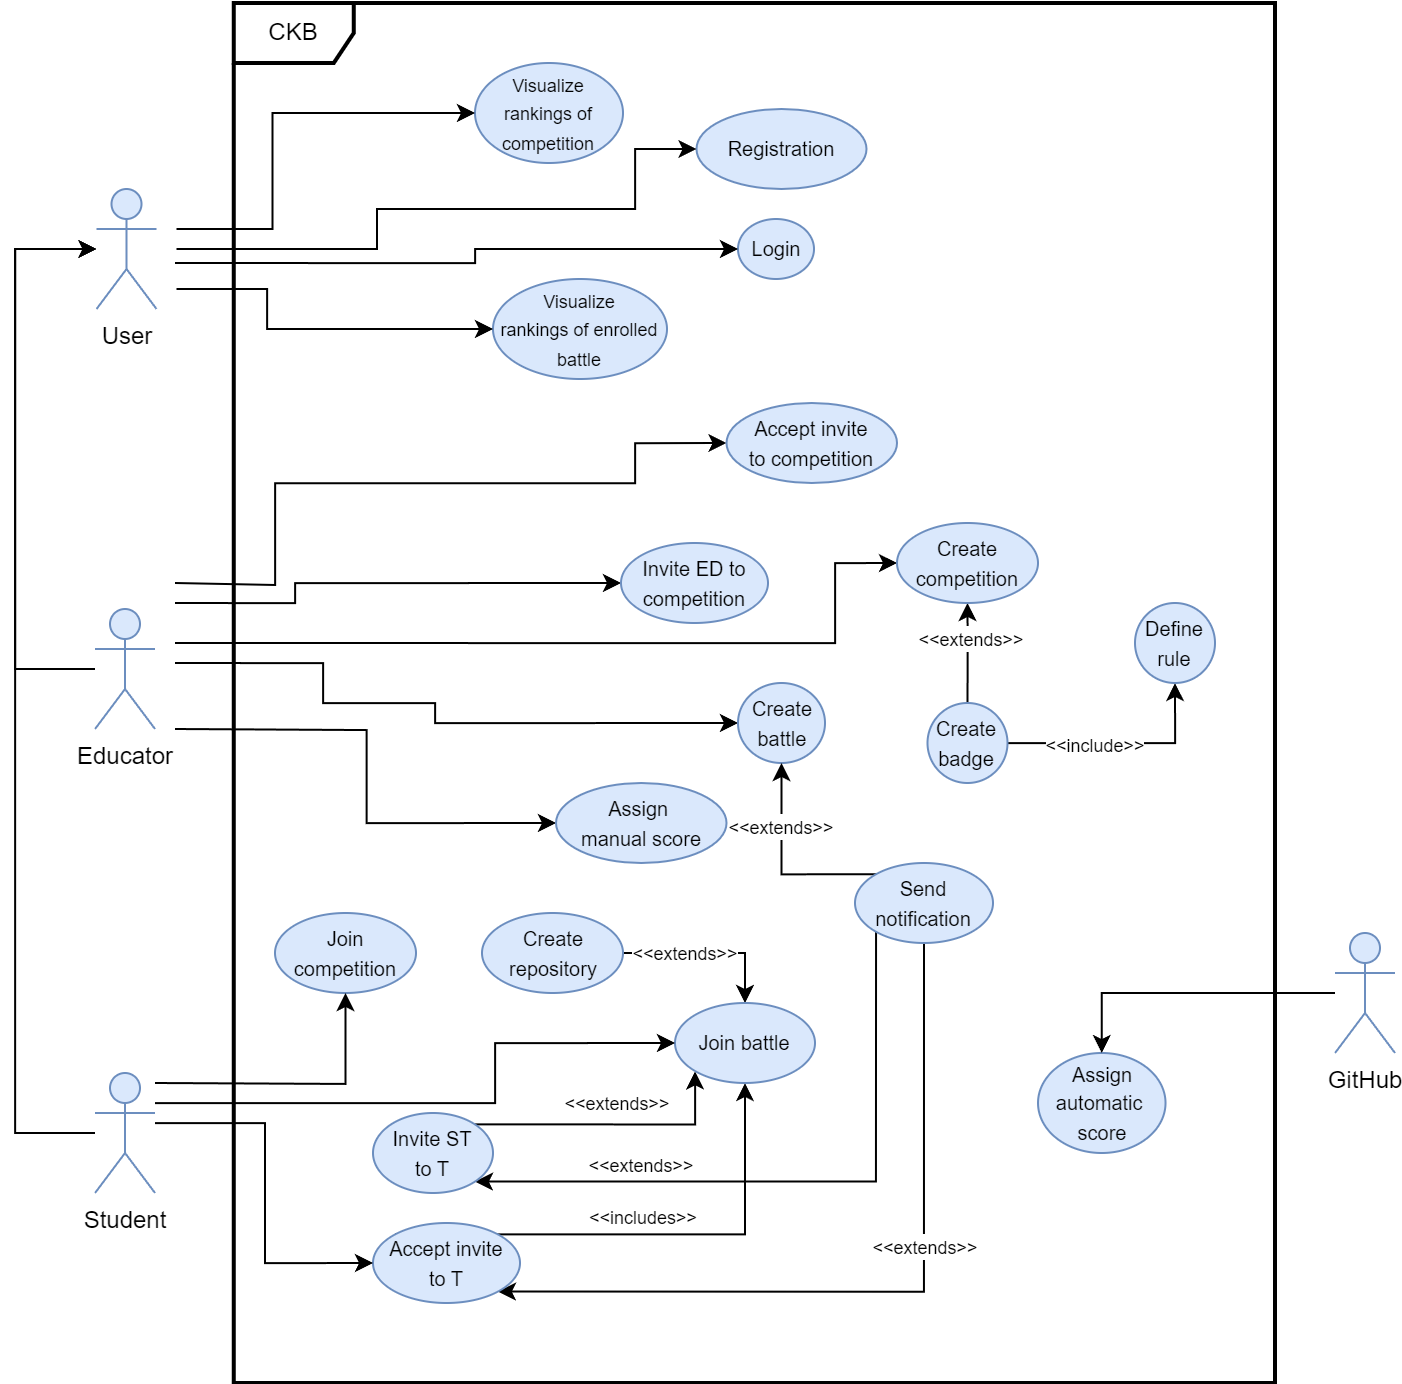
\includegraphics[width=\textwidth,height=\textheight,keepaspectratio]{Images/RASD_UseCaseDiagram.png}
        \caption{Use case diagram of the platform.}
        \label{fig: UseCaseDiagram}
    \end{center}
  \end{figure}
\end{center}

For simplicity we decided not to include all the \textit{<<include>>} relationship related to the \textbf{\textit{Login}} use case, since  almost every use case requires the user to be logged in, this was to explain that it was not forgotten.

\subsubsection*{UC1: Unregistered ST creates an account}
\begin{center}
  \begin{longtable}{l|p{0.75\linewidth}}
    \hline
    Actor & Unregistered ST \\
    \hline
    Entry conditions & The ST isn’t already registered in the \verb|CKB| platform and he clicks on the sign-up button \\
    \hline
    Event Flow & 1.\ CKB asks the ST to insert the personal information (i.e. name, surname, nickname, e-mail and password) \\
    & 2.\ The ST fills out the form with the requested informations and accepts the “Terms \& Conditions” and “Privacy Policy” \\
    & 3.\ CKB validate the inserted information \\
    & 4.\ CKB sends an account activation link to the email inserted by the ST \\
    & 5.\ ST clicks on the link received in the email \\
    & 6.\ CKB confirms the account creation  \\
    \hline
    Exit condition & The ST account is created \\
    \hline
    Exceptions & 3.1 CKB isn’t able to validate the information inserted (i.e. duplicate email, duplicate username and wrong email address \\
    & 5.1 The link is expired \\ \\
    & In all the cases the ST is notified with an error message\\
    \hline
    \caption{ST signs up case.}
    \label{tab: ST_signs_up}
  \end{longtable}

  \begin{figure} [H]
    \begin{center}
        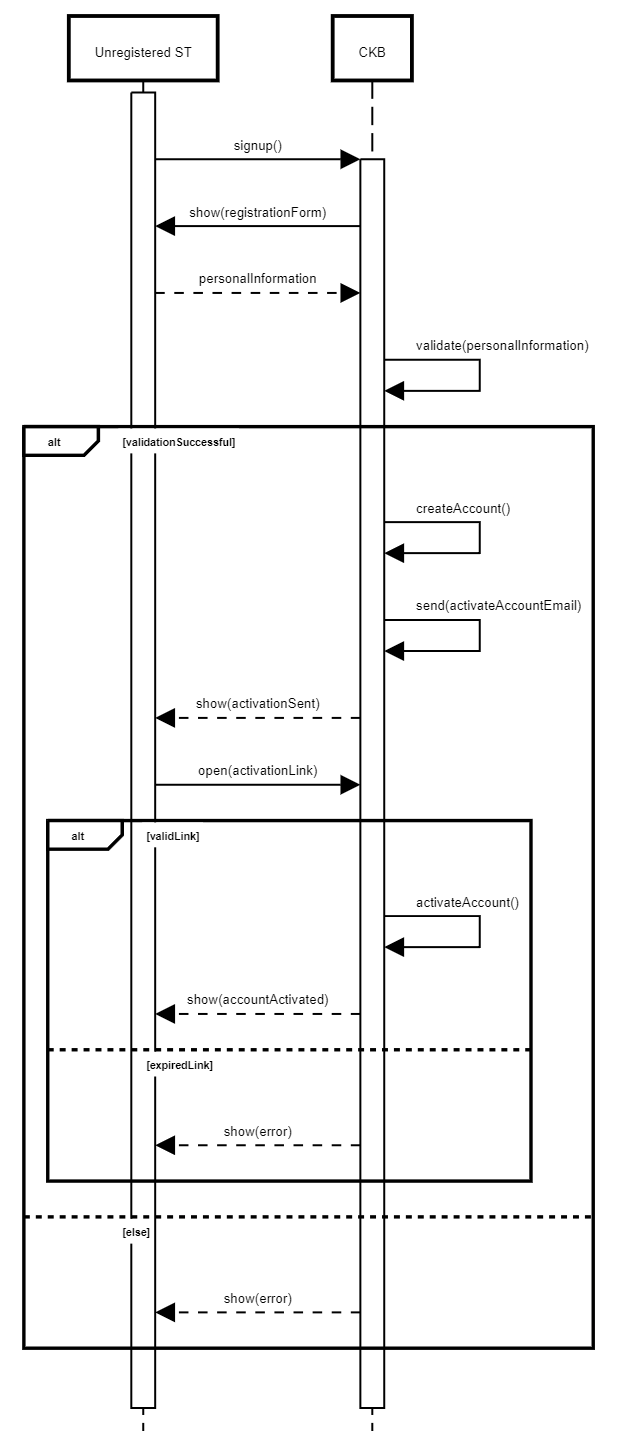
\includegraphics[width=\textwidth,height=\textheight,keepaspectratio]{Images/SequenceDiagrams/UC1.png}
        \caption{UC1 sequence diagram.}
        \label{fig: UC1_sequence_diagram}
    \end{center}
  \end{figure}
\end{center}

\subsubsection*{UC2: Unregistered ED creates an account}
\begin{center}
  \begin{longtable}{l|p{0.75\linewidth}}
    \hline
    Actor & Unregistered ED \\
    \hline
    Entry conditions & The ED isn’t already registered in the \verb|CKB| platform and he clicks on the sign-up button \\
    \hline
    Event Flow & 1.\ CKB asks the ED to insert the personal information (i.e. name, surname, nickname, e-mail and password) \\
    & 2.\ The ED fills out the form with the requested informations and accepts the “Terms \& Conditions” and “Privacy Policy” \\
    & 3.\ CKB validate the inserted information \\
    & 4.\ CKB asks the ED to insert the information about the institution (i.e. name, address, city, country, website) \\
    & 5.\ The ED fills out the form with the requested informations \\
    & 6.\ CKB validate the information about the institute \\
    & 7.\ CKB sends an account activation link to the email inserted by the ED \\
    & 8.\ ED clicks on the link received in the email \\
    & 9.\ CKB confirms the account creation  \\
    \hline
    Exit condition & The ED account is created \\
    \hline
    Exceptions & 3.1 CKB isn’t able to validate the information inserted (i.e. duplicate email, duplicate username and wrong email address \\
    & 6.1 CKB isn’t able to validate the information about the institute \\
    & 8.1 The link is expired \\ \\
    & In all the cases the ST is notified with an error message\\
    \hline
    \caption{ED signs up case.}
    \label{tab: ED_signs_up}
  \end{longtable}

  \begin{figure} [H]
    \begin{center}
        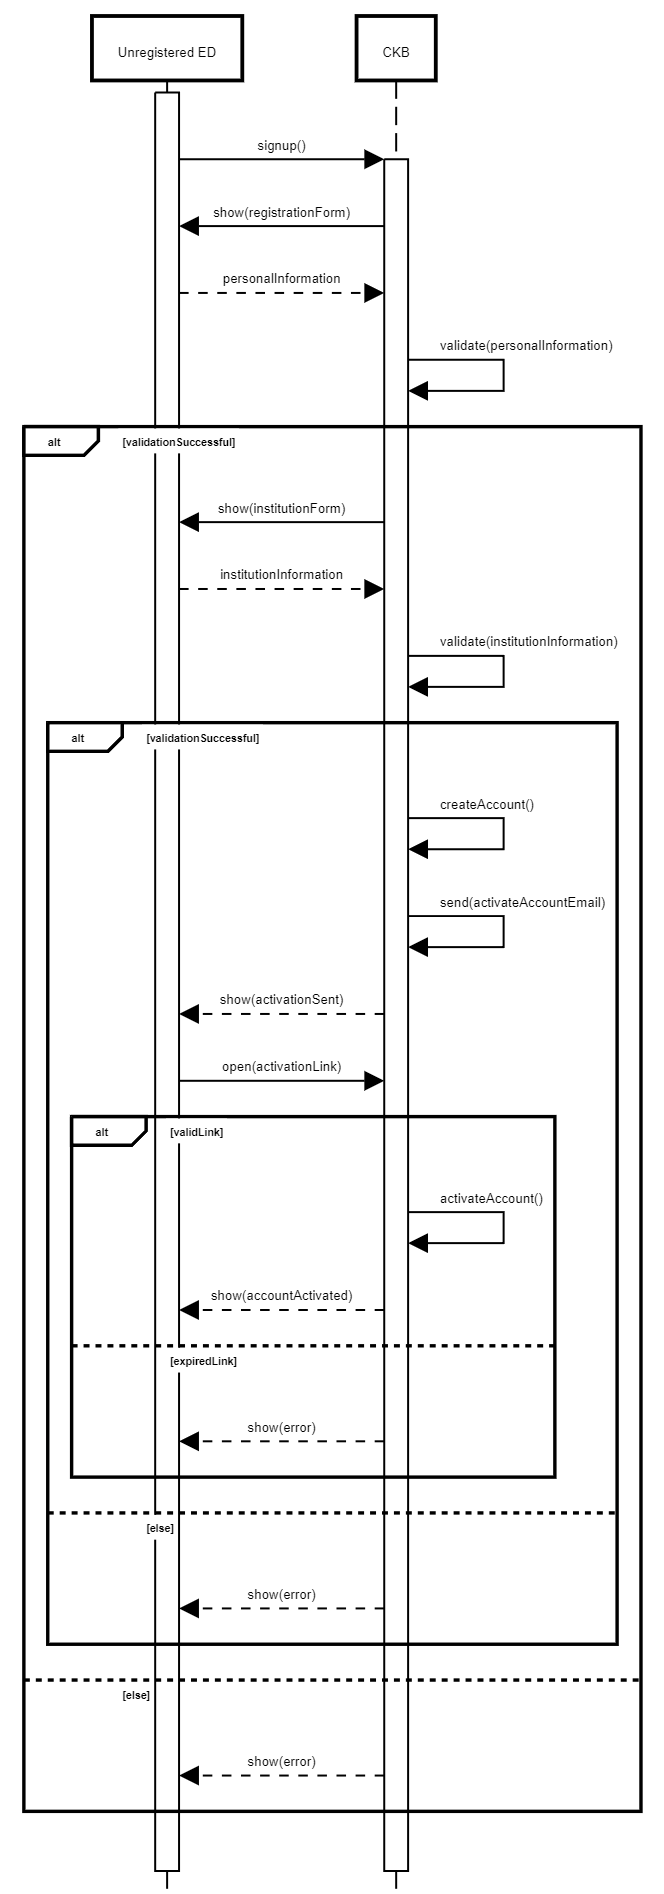
\includegraphics[width=\textwidth,height=\textheight,keepaspectratio]{Images/SequenceDiagrams/UC2.png}
        \caption{UC2 sequence diagram.}
        \label{fig: UC2_sequence_diagram}
    \end{center}
  \end{figure}
\end{center}

\subsubsection*{UC3: ST or ED logs in}
\begin{center}
  \begin{longtable}{l|p{0.75\linewidth}}
    \hline
    Actor & Registered ST \\
    & Registered ED \\
    \hline
    Entry conditions & The ED isn already registered in the \verb|CKB| platform \\
    \hline
    Event Flow & 1.\ The user clicks on the login button \\
    & 2.\ CKB asks for the username and the password \\
    & 3.\ The user inserts the username and the password \\
    & 4.\ CKB validates the information \\
    & 5.\ CKB redirects the user to the home page \\
    \hline
    Exit condition & The user is logged in \\
    \hline
    Exceptions & 4.1 The username or the password are wrong \\ \\
    & In this case the user is notified with an error message \\
    \hline
    \caption{ST or ED logs in.}
    \label{tab: ST_or_ED_logs_in}
  \end{longtable}

  \begin{figure} [H]
    \begin{center}
        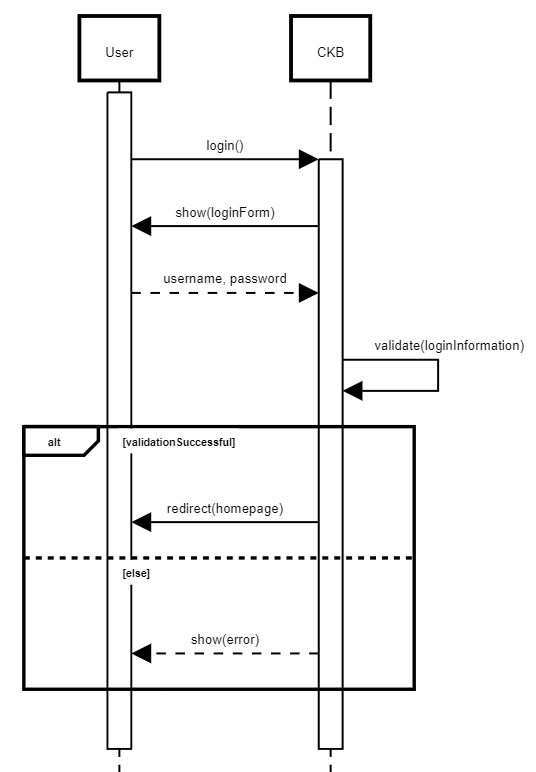
\includegraphics[width=0.65\textwidth,height=\textheight,keepaspectratio]{Images/SequenceDiagrams/UC3.png}
        \caption{UC3 sequence diagram.}
        \label{fig: UC3_sequence_diagram}
    \end{center}
  \end{figure}
\end{center}

\subsubsection*{UC4: ED creates a new competition}
\begin{center}
  \begin{longtable}{l|p{0.75\linewidth}}
    \hline
    Actor & Registered ED \\
    \hline
    Entry conditions & The ED is already registered and logged in  \\
    & The ED clicks on the “Create Competition” button \\
    \hline
    Event Flow & 1.\ CKB asks for a name for the competition \\
    & 2.\ The ED inserts the name \\
    & 3.\ CKB checks if the name is available \\
    & 4.\ CKB asks for the information of the competition (i.e. description, start date, end date, programming languages allowed) \\
    & 5.\ CKB validates the information \\
    & 6.\ CKB creates the competition \\
    \hline
    Exit condition & The competition is correctly created \\
    \hline
    Exceptions & 3.1 The name is already used by another competition \\
    & 5.1 CKB isn’t able to validate the information \\ \\
    & In the first case the ED is notified with an error message and the flow restarts from the step 1 \\
    & In the other case the ED is notified with an error message \\
    \hline
    \caption{ED creates a competiton.}
    \label{tab: ED_create_competition}
  \end{longtable}

  \begin{figure} [H]
    \begin{center}
        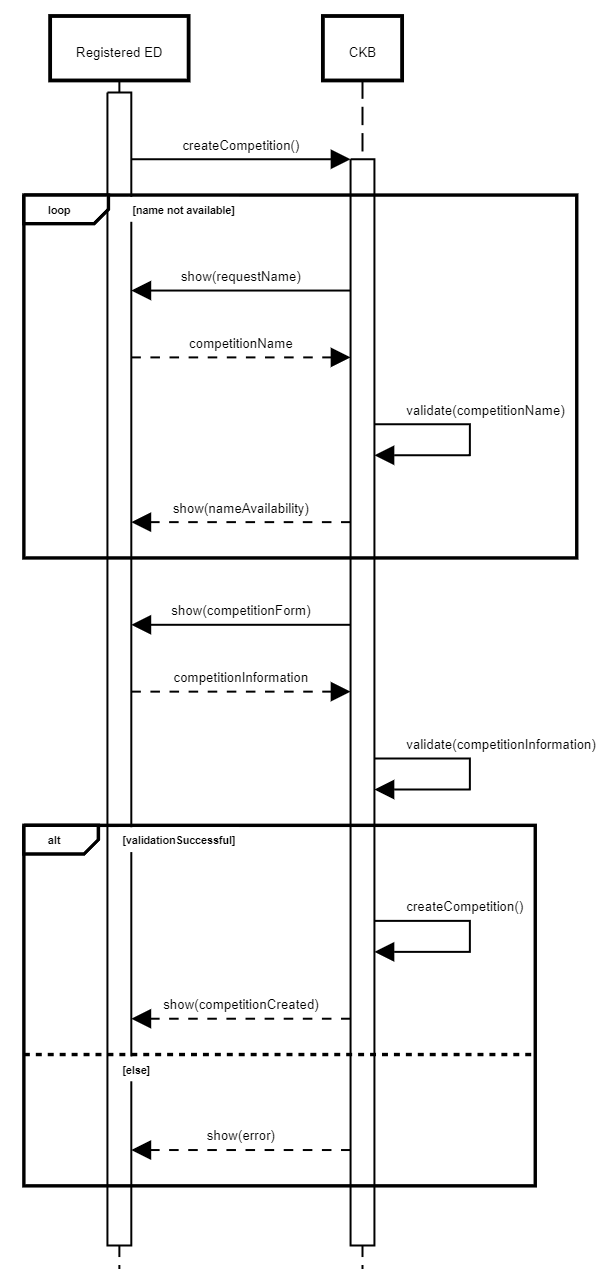
\includegraphics[width=\textwidth,height=\textheight,keepaspectratio]{Images/SequenceDiagrams/UC4.png}
        \caption{UC4 sequence diagram.}
        \label{fig: UC4_sequence_diagram}
    \end{center}
  \end{figure}
\end{center}

\subsubsection*{UC5: ST joins a competition}
\begin{center}
  \begin{longtable}{l|p{0.75\linewidth}}
    \hline
    Actor & Registered ST \\
    \hline
    Entry conditions & The ST is already registered and logged in  \\
    \hline
    Event Flow & 1.\ CKB shows the list of the available competitions \\
    & 2.\ The ST selects the competition \\
    & 3.\ CKB shows the information about the competition \\
    & 4.\ The ST clicks on the “Join” button \\
    & 5.\ CKB adds the ST to the competition \\
    & 6.\ ST can now see the competition in the “My Competitions” section \\
    \hline
    Exit condition & The ST has joined the competition \\
    \hline
    Exceptions & 2.1 There are no competitions available \\ \\
    & In this case the ST visualizes a message that there are no competition available \\ \\
    \hline
    \caption{ST joins a competition.}
    \label{tab: ST_join_competition}
  \end{longtable}

  \begin{figure} [H]
    \begin{center}
        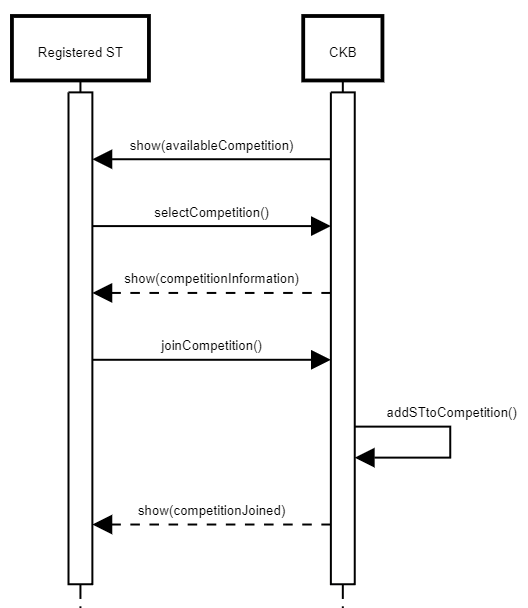
\includegraphics[width=0.65\textwidth,height=\textheight,keepaspectratio]{Images/SequenceDiagrams/UC5.png}
        \caption{UC5 sequence diagram.}
        \label{fig: UC5_sequence_diagram}
    \end{center}
  \end{figure}
\end{center}

\subsubsection*{UC6: ED creates a new battle inside a competition}
\begin{center}
  \begin{longtable}{l|p{0.75\linewidth}}
    \hline
    Actor & Registered ED \\
    \hline
    Entry conditions & The ED is already registered and logged in  \\
    & The ED is the creator or a collaborator of the competition \\
    & The ED is in the competition page \\
    & The ED clicks on the “Create Battle” button \\
    \hline
    Event Flow & 1.\ CKB asks for a name for the battle \\
    & 2.\ CKB checks if the name is not already used for another battle inside the competition \\
    & 3.\ CKB asks for the information of the battle (i.e. description, start date, end date, programming languages allowed, number of teams, number of members per team) \\
    & 4.\ ED inserts the information \\
    & 5.\ CKB asks for the configuration of the static analyzer \\
    & 6.\ CKB asks to upload the test cases and the solution \\
    & 7.\ ED uploads the files and insert all the information requested \\
    & 8.\ CKB validates the information \\
    & 9.\ CKB creates the battle \\
    \hline
    Exit condition & The battle is created correctly \\
    \hline
    Exceptions & 6.1 The upload of the files fails \\
    & 7.1 CKB isn’t able to validate the information \\ \\
    & In all the cases the ED is notified with an error message \\
    \hline
    \caption{ED creates a battle inside a competition.}
    \label{tab: ED_create_battle}
  \end{longtable}

  \begin{figure} [H]
    \begin{center}
        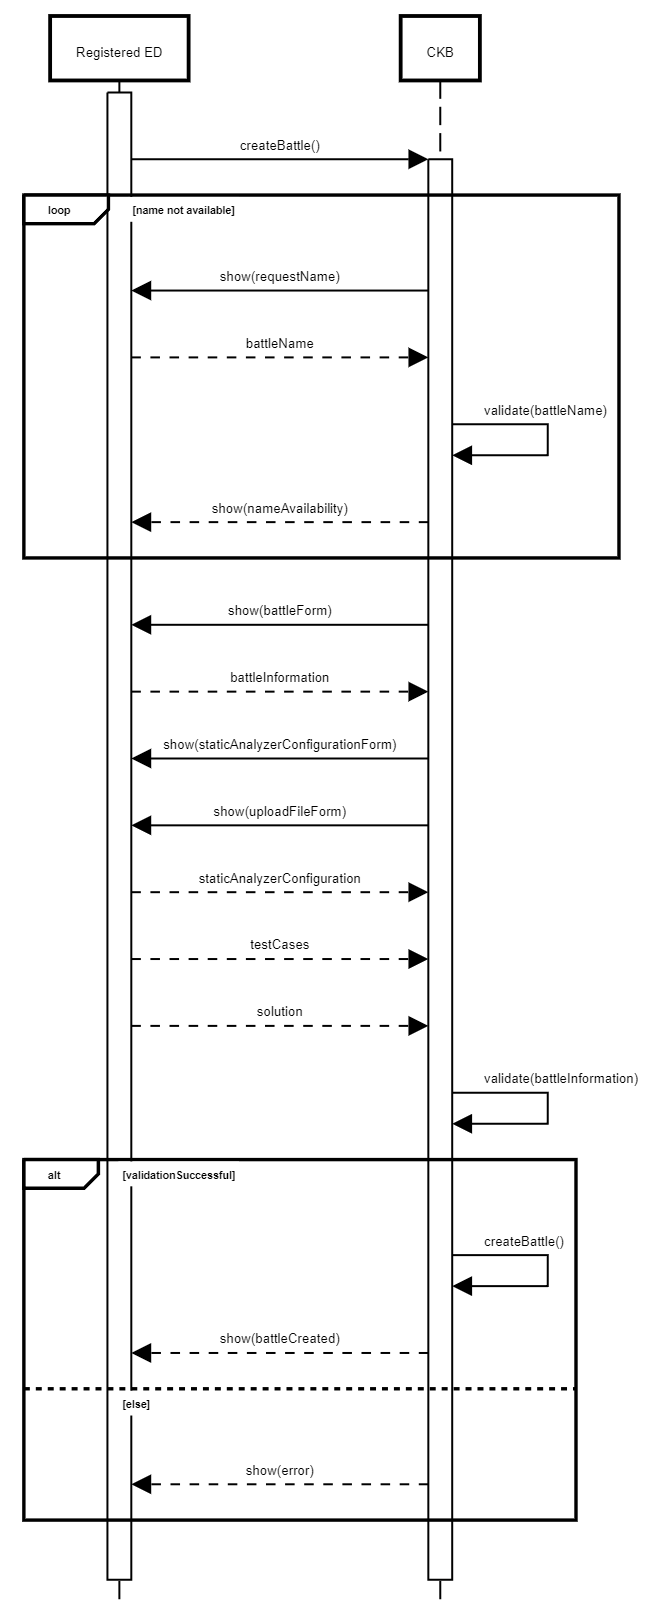
\includegraphics[width=\textwidth,height=\textheight,keepaspectratio]{Images/SequenceDiagrams/UC6.png}
        \caption{UC6 sequence diagram.}
        \label{fig: UC6_sequence_diagram}
    \end{center}
  \end{figure}
\end{center}

\subsubsection*{UC7: ED invites other EDs to a competition}
\begin{center}
  \begin{longtable}{l|p{0.75\linewidth}}
    \hline
    Actor & Registered ED \\
    \hline
    Entry conditions & The ED is already registered and logged in  \\
    & The ED is the creator or a collaborator of the competition \\
    & The ED is in the competition page \\
    \hline
    Event Flow & 1.\ ED clicks on the "Settings" button inside the competition\\
    & 2.\ ED scrolls down to the "Collaborators" section \\
    & 3.\ ED clicks on the "Invite" button \\
    & 4.\ CKB asks for the email or the username of the ED to invite \\
    & 5.\ ED inserts the email or the username \\
    & 6.\ CKB validates the information \\
    & 7.\ CKB sends an invitation email to the ED \\
    & 8.\ The invited ED clicks on the link received in the email \\
    & 9.\ CKB confirms the invitation  \\
    \hline
    Exit condition & The invited ED is a collaborator of the competition \\
    \hline
    Exceptions & 6.1 The email or the username is not valid \\
    & 8.1 The link is expired \\ \\
    & In all the cases the ED is notified with an error message \\
    \hline
    \caption{ED invites other EDs to a competition.}
    \label{tab: ED_invite_ED}
  \end{longtable}

  \begin{figure} [H]
    \begin{center}
        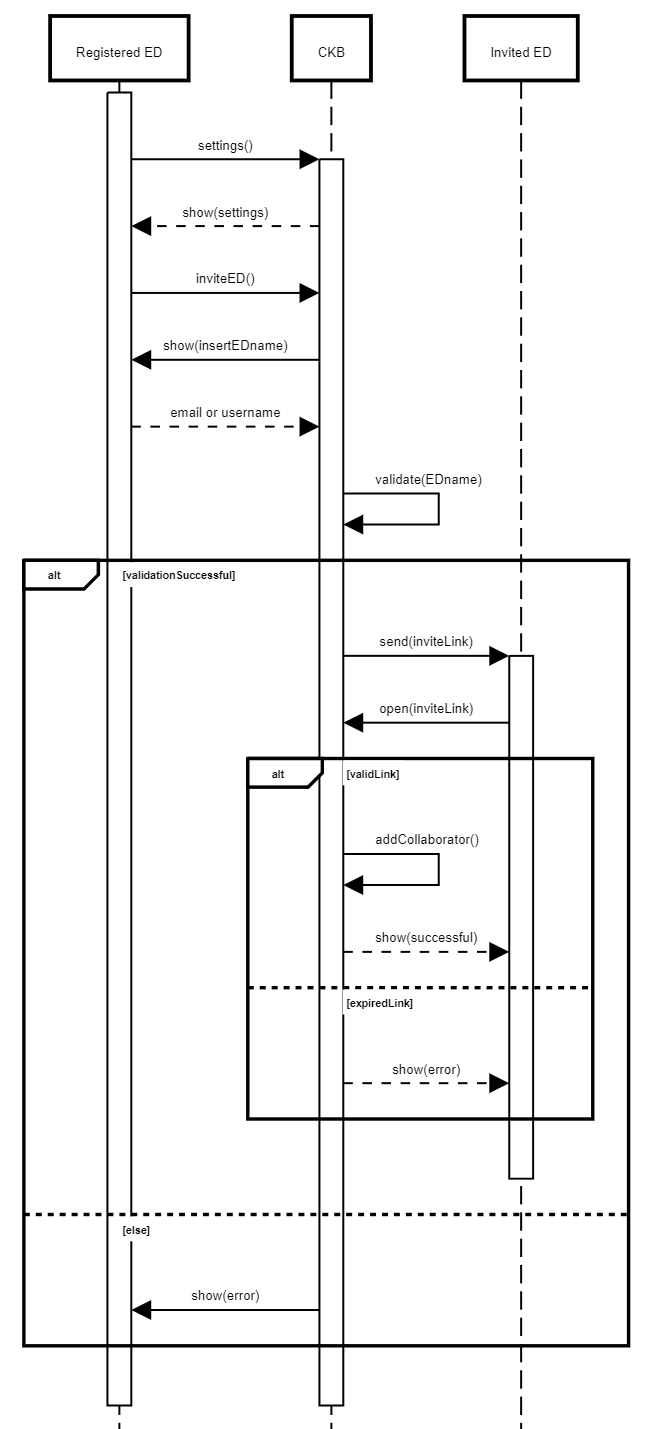
\includegraphics[width=\textwidth,height=\textheight,keepaspectratio]{Images/SequenceDiagrams/UC7.png}
        \caption{UC7 sequence diagram.}
        \label{fig: UC7_sequence_diagram}
    \end{center}
  \end{figure}
\end{center}

\subsubsection*{UC8: ED creates a new badge inside a competition}
\begin{center}
  \begin{longtable}{l|p{0.75\linewidth}}
    \hline
    Actor & Registered ED \\
    \hline
    Entry conditions & The ED is already registered and logged in  \\
    & The ED is the creator or a collaborator of the competition \\
    & The ED is in the competition page \\
    \hline
    Event Flow & 1.\ ED clicks on the "Settings" button inside the competition\\
    & 2.\ ED scrolls down to the "Badges" section \\
    & 3.\ ED clicks on the "Create new Badge" button \\
    & 4.\ CKB asks for the information (i.e. name, description) of the badge \\
    & 5.\ ED inserts the information \\
    & 6.\ CKB asks for the rules of the badge \\
    & 7.\ ED inserts the rules \\
    & 8.\ CKB validates the information \\
    & 9.\ CKB creates the badge \\
    \hline
    Exit condition &  The badge is added to the competition \\
    \hline
    Exceptions & 8.1 CKB isn’t able to validate the information \\ \\
    & The ED is notified with an error message \\
    \hline
    \caption{ED creates a badge inside a competition.}
    \label{tab: ED_create_badge}
  \end{longtable}

  \begin{figure} [H]
    \begin{center}
        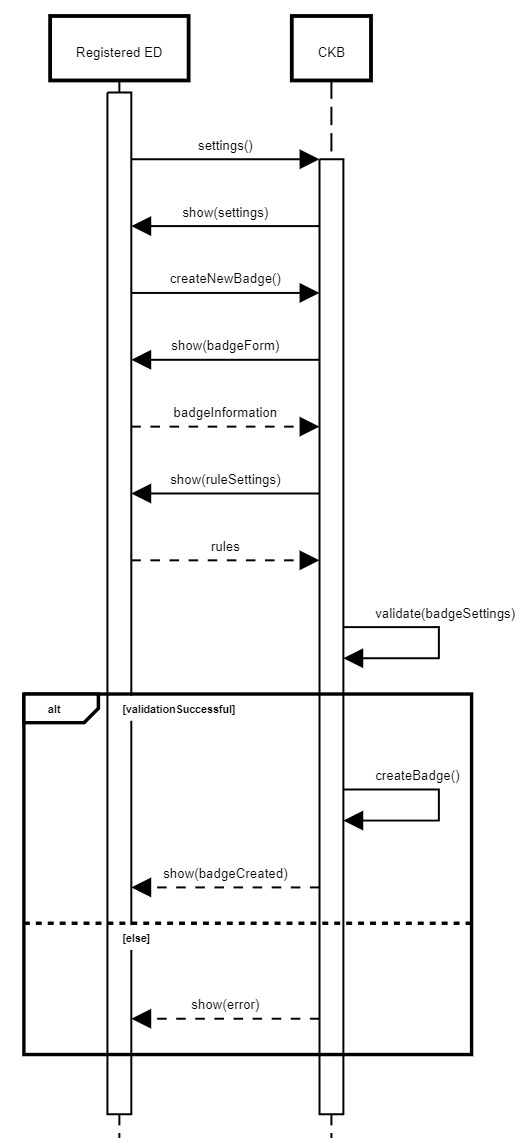
\includegraphics[width=\textwidth,height=\textheight,keepaspectratio]{Images/SequenceDiagrams/UC8.png}
        \caption{UC8 sequence diagram.}
        \label{fig: UC8_sequence_diagram}
    \end{center}
  \end{figure}
\end{center}

\subsubsection*{UC9: ST receives notification from CKB}
\begin{center}
  \begin{longtable}{l|p{0.75\linewidth}}
    \hline
    Actor & Registered ST \\
    \hline
    Entry conditions & The ST is already registered  \\
    & A competition is created \\
    & A battle inside a competiton in which the ST is enrolled is created \\
    & A battle in which the ST has partecipated has ended \\
    & The rank of a competition in which the ST has partecipated is available \\
    \hline
    Event Flow & 1.\ CKB sends a notification via email to the ST \\
    & 2.\ The ST clicks on the link received in the email \\
    & 3.\ CKB shows the information about the notification \\
    \hline
    Exit condition &  The ST received the notification \\
    \hline
    Exceptions & 2.1 The link is wrong \\ \\
    & In this case the ST is notified with an error message \\
    \hline
    \caption{ST receives notification from CKB.}
    \label{tab: ST_receive_notification}
  \end{longtable}

  \begin{figure} [H]
    \begin{center}
        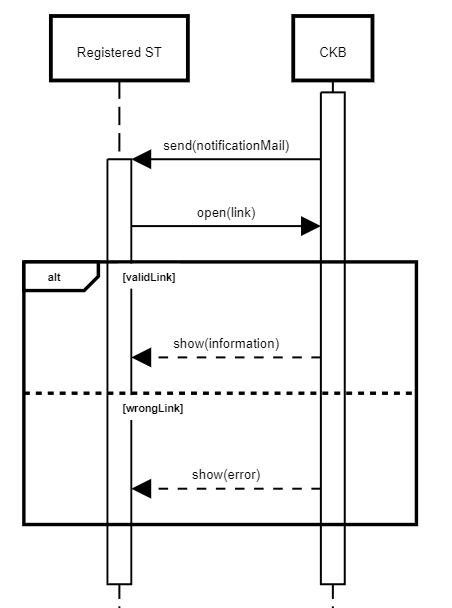
\includegraphics[width=0.65\textwidth,height=\textheight,keepaspectratio]{Images/SequenceDiagrams/UC9.png}
        \caption{UC9 sequence diagram.}
        \label{fig: UC9_sequence_diagram}
    \end{center}
  \end{figure}
\end{center}

\subsubsection*{UC10: ST visualizes the ranking of their T}
\begin{center}
  \begin{longtable}{l|p{0.75\linewidth}}
    \hline
    Actor & Registered ST \\
    \hline
    Entry conditions & The ST is already registered and logged in \\
    & The ST is enrolled in a competition \\
    & The ST is enrolled in a battle \\
    & The ST is in the competition page \\
    \hline
    Event Flow & 1.\ CKB shows the list of the battles in which the ST is enrolled \\
    & 2.\ The ST selects the battle \\
    & 3.\ The ST goes to the “Ranking” section \\
    & 4.\ CKB shows the ranking of the battle \\
    \hline
    Exit condition &  The ST visualize the ranking of their team \\
    \hline
    Exceptions & 2.1 There are no battles available \\ \\
    & In this case the ST visualizes a message that there are no battles available \\
    \hline
    \caption{ST visualizes the ranking of their T.}
    \label{tab: ST_visualize_ranking}
  \end{longtable}

  \begin{figure} [H]
    \begin{center}
        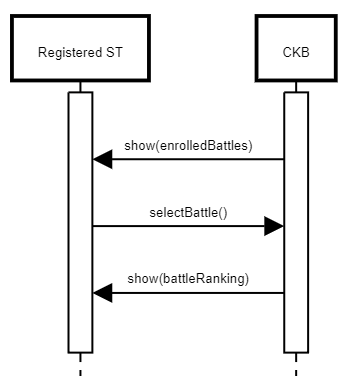
\includegraphics[width=0.5\textwidth,height=\textheight,keepaspectratio]{Images/SequenceDiagrams/UC10.png}
        \caption{UC10 sequence diagram.}
        \label{fig: UC10_sequence_diagram}
    \end{center}
  \end{figure}
\end{center}

\newpage

\subsubsection*{UC11: ED manually evaluates the code}
\begin{center}
  \begin{longtable}{l|p{0.75\linewidth}}
    \hline
    Actor & Registered ED \\
    \hline
    Entry conditions & The ED is already registered  \\
    & The ED is the creator or a collaborator of the competition \\
    & The ED is in the battle page \\
    \hline
    Event Flow & 1.\ ED clicks on a T name \\
    & 2.\ CKB shows the information about the T \\
    & 3.\ ED clicks on the “Evaluate” button \\
    & 4.\ CKB shows the information about the last code submission \\
    & 5.\ ED navigates through the code \\
    & 6.\ ED assigns a score to the code \\
    & 7.\ CKB saves the score \\
    \hline
    Exit condition &  The score is saved \\
    \hline
    Exceptions & 4.1 The T didn't submit any code \\
    & 7.1 CKB isn’t able to save the score \\ \\
    & In the first case the ED visualize a message that there are no code submissions \\
    & In the other case the ED is notified with an error message \\
    \hline
    \caption{ED manually evaluates the code.}
    \label{tab: ED_evaluate_code}
  \end{longtable}

  \begin{figure} [H]
    \begin{center}
        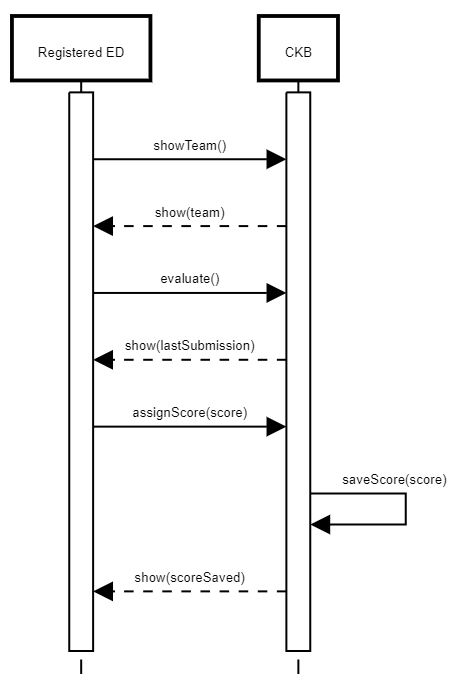
\includegraphics[width=0.65\textwidth,height=\textheight,keepaspectratio]{Images/SequenceDiagrams/UC11.png}
        \caption{UC11 sequence diagram.}
        \label{fig: UC11_sequence_diagram}
    \end{center}
  \end{figure}
\end{center}


\section{Performance Requirements}
\label{s:Performance_requirements}%

\section{Design Constraints}
\label{s:Design_constraints}%





%-------------------------------------------------------------------------
%	Formal Analysis Using Alloy
%-------------------------------------------------------------------------
\chapter{Formal Analysis Using Alloy}
\label{c:alloy}%
In our formal analysis, we deliberately focused on highlighting various snapshots that capture the intricate representation of the system, opting against the utilization of Alloy 6's time features. This strategic decision stems from our dedication to modeling the inherent complexity of the problem in a more comprehensive manner. The incorporation of Alloy 6 features would have presented substantial challenges, given the heightened complexity they introduce. Moreover, it would have necessitated a compromise in the completeness of our representation, as it would require reducing the intricacy to accommodate the depiction of time evolution.

\section{Alloy Code}
\lstinputlisting[language=alloy]{alloy/CKB_alloy.als}

\section{Assertion Results}

\begin{figure}[H]
    \centering
    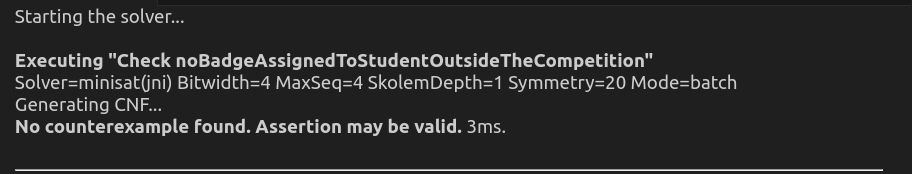
\includegraphics[width=200px]{Images/alloy/assert_1.png}
    \caption{Assert there is no student part of a battle for a competition it did not join}
\end{figure}

\begin{figure}[H]
    \centering
    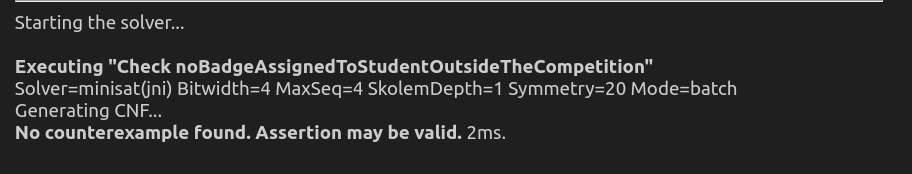
\includegraphics[width=200px]{Images/alloy/assert_2.png}
    \caption{Assert there is no started battle with waiting teams inside}
\end{figure}

\begin{figure}[H]
    \centering
    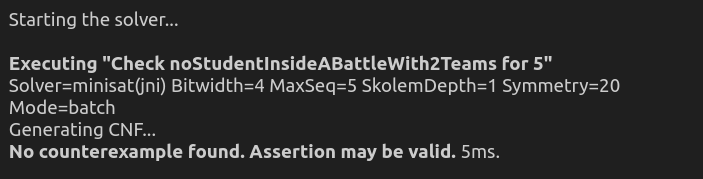
\includegraphics[width=200px]{Images/alloy/assert_3.png}
    \caption{Assert there is no student isnide a battle with 2 teams}
\end{figure}


\begin{figure}[H]
    \centering
    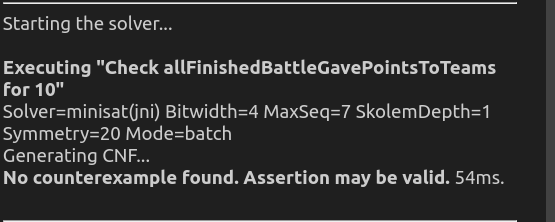
\includegraphics[width=200px]{Images/alloy/assert_4.png}
    \caption{Assert all finish battle gave points to the teams}
\end{figure}

\section{World Generated}


%-------------------------------------------------------------------------
%	Effort Spent
%-------------------------------------------------------------------------
\chapter{Effort Spent}
\label{c:effort}%
\begin{table}[H]
  \centering
  \begin{tabular}{|l|l|}
    \hline
    \textbf{Members of group} & \textbf{Effort spent (hours)} \\ 
    \hline
    Filippo Balzarini & \begin{tabular}{p{0.25\linewidth}|c}
      Introduction          & $0h$  \\
      Architectural design  & $10h$ \\
      User interface design & $0h$ \\
      Requirements traceability      & $2h$ \\
      Implementation, integration and test plan & $2h$ \\
      Reasoning             & $2h$ \\
    \end{tabular} \\ 
    \hline
    Christian Biffi & \begin{tabular}{p{0.25\linewidth}|c}
      Introduction          & $1h$  \\
      Architectural design  & $6h$ \\
      User interface design & $8h$ \\
      Requirements traceability      & $0h$ \\
      Implementation, integration and test plan & $0h$ \\
      Reasoning             & $4h$ \\
    \end{tabular} \\ 
    \hline
    Michele Cavicchioli & \begin{tabular}{p{0.25\linewidth}|c}
      Introduction          & $1h$  \\
      Architectural design  & $9h$ \\
      User interface design & $0h$ \\
      Requirements traceability      & $1h$ \\
      Implementation, integration and test plan & $2h$ \\
      Reasoning             & $5h$ \\
    \end{tabular} \\ 
    \hline
  \end{tabular}
  \caption{Effort spent by each member of the group}
  \label{tab:effortSpent}
\end{table}



%-------------------------------------------------------------------------
%	BIBLIOGRAPHY
%-------------------------------------------------------------------------

\addtocontents{toc}{\vspace{2em}} % Add a gap in the Contents, for aesthetics
\bibliography{RASD_bibliography} % The references information are stored in the file named "Thesis_bibliography.bib"

%-------------------------------------------------------------------------
%	APPENDICES
%-------------------------------------------------------------------------

\cleardoublepage
\addtocontents{toc}{\vspace{2em}} % Add a gap in the Contents, for aesthetics
\appendix

% LIST OF FIGURES
\listoffigures

% LIST OF TABLES
\listoftables

% LIST OF SYMBOLS
% Write out the List of Symbols in this page
\chapter*{List of Symbols} % You have to include a chapter for your list of symbols (
\begin{table}[H]
    \centering
    \begin{tabular}{lll}
        \textbf{Variable} & \textbf{Description} & \textbf{SI unit} \\\hline\\[-9px]
        $\bm{u}$ & solid displacement & m \\[2px]
        $\bm{u}_f$ & fluid displacement & m \\[2px]
    \end{tabular}
\end{table}


\cleardoublepage

\end{document}
